
%% bare_adv.tex
%% V1.4b
%% 2015/08/26
%% by Michael Shell
%% See:
%% http://www.michaelshell.org/
%% for current contact information.
%%
%% This is a skeleton file demonstrating the advanced use of IEEEtran.cls
%% (requires IEEEtran.cls version 1.8b or later) with an IEEE Computer
%% Society journal paper.
%%
%% Support sites:
%% http://www.michaelshell.org/tex/ieeetran/
%% http://www.ctan.org/pkg/ieeetran
%% and
%% http://www.ieee.org/

%%*************************************************************************
%% Legal Notice:
%% This code is offered as-is without any warranty either expressed or
%% implied; without even the implied warranty of MERCHANTABILITY or
%% FITNESS FOR A PARTICULAR PURPOSE!
%% User assumes all risk.
%% In no event shall the IEEE or any contributor to this code be liable for
%% any damages or losses, including, but not limited to, incidental,
%% consequential, or any other damages, resulting from the use or misuse
%% of any information contained here.
%%
%% All comments are the opinions of their respective authors and are not
%% necessarily endorsed by the IEEE.
%%
%% This work is distributed under the LaTeX Project Public License (LPPL)
%% ( http://www.latex-project.org/ ) version 1.3, and may be freely used,
%% distributed and modified. A copy of the LPPL, version 1.3, is included
%% in the base LaTeX documentation of all distributions of LaTeX released
%% 2003/12/01 or later.
%% Retain all contribution notices and credits.
%% ** Modified files should be clearly indicated as such, including  **
%% ** renaming them and changing author support contact information. **
%%*************************************************************************


% *** Authors should verify (and, if needed, correct) their LaTeX system  ***
% *** with the testflow diagnostic prior to trusting their LaTeX platform ***
% *** with production work. The IEEE's font choices and paper sizes can   ***
% *** trigger bugs that do not appear when using other class files.       ***                          ***
% The testflow support page is at:
% http://www.michaelshell.org/tex/testflow/


% IEEEtran V1.7 and later provides for these CLASSINPUT macros to allow the
% user to reprogram some IEEEtran.cls defaults if needed. These settings
% override the internal defaults of IEEEtran.cls regardless of which class
% options are used. Do not use these unless you have good reason to do so as
% they can result in nonIEEE compliant documents. User beware. ;)
%
%\newcommand{\CLASSINPUTbaselinestretch}{1.0} % baselinestretch
%\newcommand{\CLASSINPUTinnersidemargin}{1in} % inner side margin
%\newcommand{\CLASSINPUToutersidemargin}{1in} % outer side margin
%\newcommand{\CLASSINPUTtoptextmargin}{1in}   % top text margin
%\newcommand{\CLASSINPUTbottomtextmargin}{1in}% bottom text margin




%
\documentclass[10pt,journal,compsoc]{IEEEtran}
% If IEEEtran.cls has not been installed into the LaTeX system files,
% manually specify the path to it like:
% \documentclass[10pt,journal,compsoc]{../sty/IEEEtran}


% For Computer Society journals, IEEEtran defaults to the use of
% Palatino/Palladio as is done in IEEE Computer Society journals.
% To go back to Times Roman, you can use this code:
%\renewcommand{\rmdefault}{ptm}\selectfont





% Some very useful LaTeX packages include:
% (uncomment the ones you want to load)



% *** MISC UTILITY PACKAGES ***
%
%\usepackage{ifpdf}
% Heiko Oberdiek's ifpdf.sty is very useful if you need conditional
% compilation based on whether the output is pdf or dvi.
% usage:
% \ifpdf
%   % pdf code
% \else
%   % dvi code
% \fi
% The latest version of ifpdf.sty can be obtained from:
% http://www.ctan.org/pkg/ifpdf
% Also, note that IEEEtran.cls V1.7 and later provides a builtin
% \ifCLASSINFOpdf conditional that works the same way.
% When switching from latex to pdflatex and vice-versa, the compiler may
% have to be run twice to clear warning/error messages.






% *** CITATION PACKAGES ***
%
\ifCLASSOPTIONcompsoc
  % The IEEE Computer Society needs nocompress option
  % requires cite.sty v4.0 or later (November 2003)
  \usepackage[nocompress]{cite}
\else
  % normal IEEE
  \usepackage{cite}
\fi
% cite.sty was written by Donald Arseneau
% V1.6 and later of IEEEtran pre-defines the format of the cite.sty package
% \cite{} output to follow that of the IEEE. Loading the cite package will
% result in citation numbers being automatically sorted and properly
% "compressed/ranged". e.g., [1], [9], [2], [7], [5], [6] without using
% cite.sty will become [1], [2], [5]--[7], [9] using cite.sty. cite.sty's
% \cite will automatically add leading space, if needed. Use cite.sty's
% noadjust option (cite.sty V3.8 and later) if you want to turn this off
% such as if a citation ever needs to be enclosed in parenthesis.
% cite.sty is already installed on most LaTeX systems. Be sure and use
% version 5.0 (2009-03-20) and later if using hyperref.sty.
% The latest version can be obtained at:
% http://www.ctan.org/pkg/cite
% The documentation is contained in the cite.sty file itself.
%
% Note that some packages require special options to format as the Computer
% Society requires. In particular, Computer Society  papers do not use
% compressed citation ranges as is done in typical IEEE papers
% (e.g., [1]-[4]). Instead, they list every citation separately in order
% (e.g., [1], [2], [3], [4]). To get the latter we need to load the cite
% package with the nocompress option which is supported by cite.sty v4.0
% and later.





% *** GRAPHICS RELATED PACKAGES ***
%
\ifCLASSINFOpdf
   \usepackage[pdftex]{graphicx}
  % declare the path(s) where your graphic files are
  % \graphicspath{{../pdf/}{../jpeg/}}
  % and their extensions so you won't have to specify these with
  % every instance of \includegraphics
  % \DeclareGraphicsExtensions{.pdf,.jpeg,.png}
\else
  % or other class option (dvipsone, dvipdf, if not using dvips). graphicx
  % will default to the driver specified in the system graphics.cfg if no
  % driver is specified.
   \usepackage[dvips]{graphicx}
  % declare the path(s) where your graphic files are
  % \graphicspath{{../eps/}}
  % and their extensions so you won't have to specify these with
  % every instance of \includegraphics
  % \DeclareGraphicsExtensions{.eps}
\fi
% graphicx was written by David Carlisle and Sebastian Rahtz. It is
% required if you want graphics, photos, etc. graphicx.sty is already
% installed on most LaTeX systems. The latest version and documentation
% can be obtained at:
% http://www.ctan.org/pkg/graphicx
% Another good source of documentation is "Using Imported Graphics in
% LaTeX2e" by Keith Reckdahl which can be found at:
% http://www.ctan.org/pkg/epslatex
%
% latex, and pdflatex in dvi mode, support graphics in encapsulated
% postscript (.eps) format. pdflatex in pdf mode supports graphics
% in .pdf, .jpeg, .png and .mps (metapost) formats. Users should ensure
% that all non-photo figures use a vector format (.eps, .pdf, .mps) and
% not a bitmapped formats (.jpeg, .png). The IEEE frowns on bitmapped formats
% which can result in "jaggedy"/blurry rendering of lines and letters as
% well as large increases in file sizes.
%
% You can find documentation about the pdfTeX application at:
% http://www.tug.org/applications/pdftex





% *** MATH PACKAGES ***
%
\usepackage{amsmath}
\usepackage{listings}% use mathematical symbols in Verbatim environment
\lstset{
  basicstyle=\ttfamily,
  mathescape
}


% A popular package from the American Mathematical Society that provides
% many useful and powerful commands for dealing with mathematics.
%
% Note that the amsmath package sets \interdisplaylinepenalty to 10000
% thus preventing page breaks from occurring within multiline equations. Use:
%\interdisplaylinepenalty=2500
% after loading amsmath to restore such page breaks as IEEEtran.cls normally
% does. amsmath.sty is already installed on most LaTeX systems. The latest
% version and documentation can be obtained at:
% http://www.ctan.org/pkg/amsmath





% *** SPECIALIZED LIST PACKAGES ***
%\usepackage{acronym}
% acronym.sty was written by Tobias Oetiker. This package provides tools for
% managing documents with large numbers of acronyms. (You don't *have* to
% use this package - unless you have a lot of acronyms, you may feel that
% such package management of them is bit of an overkill.)
% Do note that the acronym environment (which lists acronyms) will have a
% problem when used under IEEEtran.cls because acronym.sty relies on the
% description list environment - which IEEEtran.cls has customized for
% producing IEEE style lists. A workaround is to declared the longest
% label width via the IEEEtran.cls \IEEEiedlistdecl global control:
%
% \renewcommand{\IEEEiedlistdecl}{\IEEEsetlabelwidth{SONET}}
% \begin{acronym}
%
% \end{acronym}
% \renewcommand{\IEEEiedlistdecl}{\relax}% remember to reset \IEEEiedlistdecl
%
% instead of using the acronym environment's optional argument.
% The latest version and documentation can be obtained at:
% http://www.ctan.org/pkg/acronym


%\usepackage{algorithmic}
% algorithmic.sty was written by Peter Williams and Rogerio Brito.
% This package provides an algorithmic environment fo describing algorithms.
% You can use the algorithmic environment in-text or within a figure
% environment to provide for a floating algorithm. Do NOT use the algorithm
% floating environment provided by algorithm.sty (by the same authors) or
% algorithm2e.sty (by Christophe Fiorio) as the IEEE does not use dedicated
% algorithm float types and packages that provide these will not provide
% correct IEEE style captions. The latest version and documentation of
% algorithmic.sty can be obtained at:
% http://www.ctan.org/pkg/algorithms
% Also of interest may be the (relatively newer and more customizable)
% algorithmicx.sty package by Szasz Janos:
% http://www.ctan.org/pkg/algorithmicx
\usepackage[linesnumbered,ruled,vlined]{algorithm2e}



% *** ALIGNMENT PACKAGES ***
%
\usepackage{array}
% Frank Mittelbach's and David Carlisle's array.sty patches and improves
% the standard LaTeX2e array and tabular environments to provide better
% appearance and additional user controls. As the default LaTeX2e table
% generation code is lacking to the point of almost being broken with
% respect to the quality of the end results, all users are strongly
% advised to use an enhanced (at the very least that provided by array.sty)
% set of table tools. array.sty is already installed on most systems. The
% latest version and documentation can be obtained at:
% http://www.ctan.org/pkg/array


%\usepackage{mdwmath}
%\usepackage{mdwtab}
% Also highly recommended is Mark Wooding's extremely powerful MDW tools,
% especially mdwmath.sty and mdwtab.sty which are used to format equations
% and tables, respectively. The MDWtools set is already installed on most
% LaTeX systems. The lastest version and documentation is available at:
% http://www.ctan.org/pkg/mdwtools


% IEEEtran contains the IEEEeqnarray family of commands that can be used to
% generate multiline equations as well as matrices, tables, etc., of high
% quality.


%\usepackage{eqparbox}
% Also of notable interest is Scott Pakin's eqparbox package for creating
% (automatically sized) equal width boxes - aka "natural width parboxes".
% Available at:
% http://www.ctan.org/pkg/eqparbox




% *** SUBFIGURE PACKAGES ***
%\ifCLASSOPTIONcompsoc
%  \usepackage[caption=false,font=footnotesize,labelfont=sf,textfont=sf]{subfig}
%\else
%  \usepackage[caption=false,font=footnotesize]{subfig}
%\fi
% subfig.sty, written by Steven Douglas Cochran, is the modern replacement
% for subfigure.sty, the latter of which is no longer maintained and is
% incompatible with some LaTeX packages including fixltx2e. However,
% subfig.sty requires and automatically loads Axel Sommerfeldt's caption.sty
% which will override IEEEtran.cls' handling of captions and this will result
% in non-IEEE style figure/table captions. To prevent this problem, be sure
% and invoke subfig.sty's "caption=false" package option (available since
% subfig.sty version 1.3, 2005/06/28) as this is will preserve IEEEtran.cls
% handling of captions.
% Note that the Computer Society format requires a sans serif font rather
% than the serif font used in traditional IEEE formatting and thus the need
% to invoke different subfig.sty package options depending on whether
% compsoc mode has been enabled.
%
% The latest version and documentation of subfig.sty can be obtained at:
% http://www.ctan.org/pkg/subfig




% *** FLOAT PACKAGES ***
%
%\usepackage{fixltx2e}
% fixltx2e, the successor to the earlier fix2col.sty, was written by
% Frank Mittelbach and David Carlisle. This package corrects a few problems
% in the LaTeX2e kernel, the most notable of which is that in current
% LaTeX2e releases, the ordering of single and double column floats is not
% guaranteed to be preserved. Thus, an unpatched LaTeX2e can allow a
% single column figure to be placed prior to an earlier double column
% figure.
% Be aware that LaTeX2e kernels dated 2015 and later have fixltx2e.sty's
% corrections already built into the system in which case a warning will
% be issued if an attempt is made to load fixltx2e.sty as it is no longer
% needed.
% The latest version and documentation can be found at:
% http://www.ctan.org/pkg/fixltx2e


%\usepackage{stfloats}
% stfloats.sty was written by Sigitas Tolusis. This package gives LaTeX2e
% the ability to do double column floats at the bottom of the page as well
% as the top. (e.g., "\begin{figure*}[!b]" is not normally possible in
% LaTeX2e). It also provides a command:
%\fnbelowfloat
% to enable the placement of footnotes below bottom floats (the standard
% LaTeX2e kernel puts them above bottom floats). This is an invasive package
% which rewrites many portions of the LaTeX2e float routines. It may not work
% with other packages that modify the LaTeX2e float routines. The latest
% version and documentation can be obtained at:
% http://www.ctan.org/pkg/stfloats
% Do not use the stfloats baselinefloat ability as the IEEE does not allow
% \baselineskip to stretch. Authors submitting work to the IEEE should note
% that the IEEE rarely uses double column equations and that authors should try
% to avoid such use. Do not be tempted to use the cuted.sty or midfloat.sty
% packages (also by Sigitas Tolusis) as the IEEE does not format its papers in
% such ways.
% Do not attempt to use stfloats with fixltx2e as they are incompatible.
% Instead, use Morten Hogholm'a dblfloatfix which combines the features
% of both fixltx2e and stfloats:
%
% \usepackage{dblfloatfix}
% The latest version can be found at:
% http://www.ctan.org/pkg/dblfloatfix


%\ifCLASSOPTIONcaptionsoff
%  \usepackage[nomarkers]{endfloat}
% \let\MYoriglatexcaption\caption
% \renewcommand{\caption}[2][\relax]{\MYoriglatexcaption[#2]{#2}}
%\fi
% endfloat.sty was written by James Darrell McCauley, Jeff Goldberg and
% Axel Sommerfeldt. This package may be useful when used in conjunction with
% IEEEtran.cls'  captionsoff option. Some IEEE journals/societies require that
% submissions have lists of figures/tables at the end of the paper and that
% figures/tables without any captions are placed on a page by themselves at
% the end of the document. If needed, the draftcls IEEEtran class option or
% \CLASSINPUTbaselinestretch interface can be used to increase the line
% spacing as well. Be sure and use the nomarkers option of endfloat to
% prevent endfloat from "marking" where the figures would have been placed
% in the text. The two hack lines of code above are a slight modification of
% that suggested by in the endfloat docs (section 8.4.1) to ensure that
% the full captions always appear in the list of figures/tables - even if
% the user used the short optional argument of \caption[]{}.
% IEEE papers do not typically make use of \caption[]'s optional argument,
% so this should not be an issue. A similar trick can be used to disable
% captions of packages such as subfig.sty that lack options to turn off
% the subcaptions:
% For subfig.sty:
% \let\MYorigsubfloat\subfloat
% \renewcommand{\subfloat}[2][\relax]{\MYorigsubfloat[]{#2}}
% However, the above trick will not work if both optional arguments of
% the \subfloat command are used. Furthermore, there needs to be a
% description of each subfigure *somewhere* and endfloat does not add
% subfigure captions to its list of figures. Thus, the best approach is to
% avoid the use of subfigure captions (many IEEE journals avoid them anyway)
% and instead reference/explain all the subfigures within the main caption.
% The latest version of endfloat.sty and its documentation can obtained at:
% http://www.ctan.org/pkg/endfloat
%
% The IEEEtran \ifCLASSOPTIONcaptionsoff conditional can also be used
% later in the document, say, to conditionally put the References on a
% page by themselves.





% *** PDF, URL AND HYPERLINK PACKAGES ***
%
\usepackage{url}
% url.sty was written by Donald Arseneau. It provides better support for
% handling and breaking URLs. url.sty is already installed on most LaTeX
% systems. The latest version and documentation can be obtained at:
% http://www.ctan.org/pkg/url
% Basically, \url{my_url_here}.


% NOTE: PDF thumbnail features are not required in IEEE papers
%       and their use requires extra complexity and work.
%\ifCLASSINFOpdf
%  \usepackage[pdftex]{thumbpdf}
%\else
%  \usepackage[dvips]{thumbpdf}
%\fi
% thumbpdf.sty and its companion Perl utility were written by Heiko Oberdiek.
% It allows the user a way to produce PDF documents that contain fancy
% thumbnail images of each of the pages (which tools like acrobat reader can
% utilize). This is possible even when using dvi->ps->pdf workflow if the
% correct thumbpdf driver options are used. thumbpdf.sty incorporates the
% file containing the PDF thumbnail information (filename.tpm is used with
% dvips, filename.tpt is used with pdftex, where filename is the base name of
% your tex document) into the final ps or pdf output document. An external
% utility, the thumbpdf *Perl script* is needed to make these .tpm or .tpt
% thumbnail files from a .ps or .pdf version of the document (which obviously
% does not yet contain pdf thumbnails). Thus, one does a:
%
% thumbpdf filename.pdf
%
% to make a filename.tpt, and:
%
% thumbpdf --mode dvips filename.ps
%
% to make a filename.tpm which will then be loaded into the document by
% thumbpdf.sty the NEXT time the document is compiled (by pdflatex or
% latex->dvips->ps2pdf). Users must be careful to regenerate the .tpt and/or
% .tpm files if the main document changes and then to recompile the
% document to incorporate the revised thumbnails to ensure that thumbnails
% match the actual pages. It is easy to forget to do this!
%
% Unix systems come with a Perl interpreter. However, MS Windows users
% will usually have to install a Perl interpreter so that the thumbpdf
% script can be run. The Ghostscript PS/PDF interpreter is also required.
% See the thumbpdf docs for details. The latest version and documentation
% can be obtained at.
% http://www.ctan.org/pkg/thumbpdf


% NOTE: PDF hyperlink and bookmark features are not required in IEEE
%       papers and their use requires extra complexity and work.
% *** IF USING HYPERREF BE SURE AND CHANGE THE EXAMPLE PDF ***
% *** TITLE/SUBJECT/AUTHOR/KEYWORDS INFO BELOW!!           ***


%personal defined packages
\usepackage{multirow,array}
% *** TABLE FOOTNOTE PACKAGES ***
\usepackage[bottom]{footmisc}
\usepackage{footnote}
\makeatletter
\def\@xfootnote[#1]{%
  \protected@xdef\@thefnmark{#1}%
  \@footnotemark\@footnotetext}
\makeatother
\usepackage{threeparttable}

\usepackage{caption}
\usepackage{subcaption}

\usepackage{placeins}

%\usepackage{subfig}

\newcommand\MYhyperrefoptions{bookmarks=true,bookmarksnumbered=true,
pdfpagemode={UseOutlines},plainpages=false,pdfpagelabels=true,
colorlinks=true,linkcolor={black},citecolor={black},urlcolor={black},
pdftitle={Bare Demo of IEEEtran.cls for Computer Society Journals},%<!CHANGE!
pdfsubject={Typesetting},%<!CHANGE!
pdfauthor={Michael D. Shell},%<!CHANGE!
pdfkeywords={Computer Society, IEEEtran, journal, LaTeX, paper,
             template}}%<^!CHANGE!
%\ifCLASSINFOpdf
%\usepackage[\MYhyperrefoptions,pdftex]{hyperref}
%\else
%\usepackage[\MYhyperrefoptions,breaklinks=true,dvips]{hyperref}
%\usepackage{breakurl}
%\fi
% One significant drawback of using hyperref under DVI output is that the
% LaTeX compiler cannot break URLs across lines or pages as can be done
% under pdfLaTeX's PDF output via the hyperref pdftex driver. This is
% probably the single most important capability distinction between the
% DVI and PDF output. Perhaps surprisingly, all the other PDF features
% (PDF bookmarks, thumbnails, etc.) can be preserved in
% .tex->.dvi->.ps->.pdf workflow if the respective packages/scripts are
% loaded/invoked with the correct driver options (dvips, etc.).
% As most IEEE papers use URLs sparingly (mainly in the references), this
% may not be as big an issue as with other publications.
%
% That said, Vilar Camara Neto created his breakurl.sty package which
% permits hyperref to easily break URLs even in dvi mode.
% Note that breakurl, unlike most other packages, must be loaded
% AFTER hyperref. The latest version of breakurl and its documentation can
% be obtained at:
% http://www.ctan.org/pkg/breakurl
% breakurl.sty is not for use under pdflatex pdf mode.
%
% The advanced features offer by hyperref.sty are not required for IEEE
% submission, so users should weigh these features against the added
% complexity of use.
% The package options above demonstrate how to enable PDF bookmarks
% (a type of table of contents viewable in Acrobat Reader) as well as
% PDF document information (title, subject, author and keywords) that is
% viewable in Acrobat reader's Document_Properties menu. PDF document
% information is also used extensively to automate the cataloging of PDF
% documents. The above set of options ensures that hyperlinks will not be
% colored in the text and thus will not be visible in the printed page,
% but will be active on "mouse over". USING COLORS OR OTHER HIGHLIGHTING
% OF HYPERLINKS CAN RESULT IN DOCUMENT REJECTION BY THE IEEE, especially if
% these appear on the "printed" page. IF IN DOUBT, ASK THE RELEVANT
% SUBMISSION EDITOR. You may need to add the option hypertexnames=false if
% you used duplicate equation numbers, etc., but this should not be needed
% in normal IEEE work.
% The latest version of hyperref and its documentation can be obtained at:
% http://www.ctan.org/pkg/hyperref





% *** Do not adjust lengths that control margins, column widths, etc. ***
% *** Do not use packages that alter fonts (such as pslatex).         ***
% There should be no need to do such things with IEEEtran.cls V1.6 and later.
% (Unless specifically asked to do so by the journal or conference you plan
% to submit to, of course. )


% correct bad hyphenation here
\hyphenation{op-tical net-works semi-conduc-tor}


\begin{document}
%
% paper title
% Titles are generally capitalized except for words such as a, an, and, as,
% at, but, by, for, in, nor, of, on, or, the, to and up, which are usually
% not capitalized unless they are the first or last word of the title.
% Linebreaks \\ can be used within to get better formatting as desired.
% Do not put math or special symbols in the title.
\title{A new approximation method for constant weight coding and its hardware implementation}
%
%
% author names and IEEE memberships
% note positions of commas and nonbreaking spaces ( ~ ) LaTeX will not break
% a structure at a ~ so this keeps an author's name from being broken across
% two lines.
% use \thanks{} to gain access to the first footnote area
% a separate \thanks must be used for each paragraph as LaTeX2e's \thanks
% was not built to handle multiple paragraphs
%
%
%\IEEEcompsocitemizethanks is a special \thanks that produces the bulleted
% lists the Computer Society journals use for "first footnote" author
% affiliations. Use \IEEEcompsocthanksitem which works much like \item
% for each affiliation group. When not in compsoc mode,
% \IEEEcompsocitemizethanks becomes like \thanks and
% \IEEEcompsocthanksitem becomes a line break with idention. This
% facilitates dual compilation, although admittedly the differences in the
% desired content of \author between the different types of papers makes a
% one-size-fits-all approach a daunting prospect. For instance, compsoc
% journal papers have the author affiliations above the "Manuscript
% received ..."  text while in non-compsoc journals this is reversed. Sigh.
\author{Jingwei Hu, Ray C.C. Cheung~\IEEEmembership{Member,~IEEE}, Tim Guneysu~\IEEEmembership{Member,~IEEE}
        %and~Jane~Doe,~\IEEEmembership{Life~Fellow,~IEEE}% <-this % stops a space
\thanks{J. Hu and R. Cheung are with the Department
of Electronic Engineering, City University of Hong Kong, Hong Kong e-mail:~j.hu@my.cityu.edu.hk; r.cheung@cityu.edu.hk.
T. Guneysu is with the Department of Mathematics and Computer Science, University of Bremen, Germany e-mail: ~tim.gueneysu@uni-bremen.de}
\thanks{Manuscript received XX XX, 2016; revised XX XX, 2016.}
}

% note the % following the last \IEEEmembership and also \thanks -
% these prevent an unwanted space from occurring between the last author name
% and the end of the author line. i.e., if you had this:
%
% \author{....lastname \thanks{...} \thanks{...} }
%                     ^------------^------------^----Do not want these spaces!
%
% a space would be appended to the last name and could cause every name on that
% line to be shifted left slightly. This is one of those "LaTeX things". For
% instance, "\textbf{A} \textbf{B}" will typeset as "A B" not "AB". To get
% "AB" then you have to do: "\textbf{A}\textbf{B}"
% \thanks is no different in this regard, so shield the last } of each \thanks
% that ends a line with a % and do not let a space in before the next \thanks.
% Spaces after \IEEEmembership other than the last one are OK (and needed) as
% you are supposed to have spaces between the names. For what it is worth,
% this is a minor point as most people would not even notice if the said evil
% space somehow managed to creep in.



% The paper headers
%\markboth{Journal of \LaTeX\ Class Files,~Vol.~14, No.~8, August~2015}%
%{Shell \MakeLowercase{\textit{et al.}}: Bare Advanced Demo of IEEEtran.cls for IEEE Computer Society Journals}
% The only time the second header will appear is for the odd numbered pages
% after the title page when using the twoside option.
%
% *** Note that you probably will NOT want to include the author's ***
% *** name in the headers of peer review papers.                   ***
% You can use \ifCLASSOPTIONpeerreview for conditional compilation here if
% you desire.



% The publisher's ID mark at the bottom of the page is less important with
% Computer Society journal papers as those publications place the marks
% outside of the main text columns and, therefore, unlike regular IEEE
% journals, the available text space is not reduced by their presence.
% If you want to put a publisher's ID mark on the page you can do it like
% this:
%\IEEEpubid{0000--0000/00\$00.00~\copyright~2015 IEEE}
% or like this to get the Computer Society new two part style.
%\IEEEpubid{\makebox[\columnwidth]{\hfill 0000--0000/00/\$00.00~\copyright~2015 IEEE}%
%\hspace{\columnsep}\makebox[\columnwidth]{Published by the IEEE Computer Society\hfill}}
% Remember, if you use this you must call \IEEEpubidadjcol in the second
% column for its text to clear the IEEEpubid mark (Computer Society journal
% papers don't need this extra clearance.)



% use for special paper notices
%\IEEEspecialpapernotice{(Invited Paper)}



% for Computer Society papers, we must declare the abstract and index terms
% PRIOR to the title within the \IEEEtitleabstractindextext IEEEtran
% command as these need to go into the title area created by \maketitle.
% As a general rule, do not put math, special symbols or citations
% in the abstract or keywords.
\IEEEtitleabstractindextext{%
\begin{abstract}
We present here a more memory efficient method for encoding binary information
into words of prescribed length and weight. Existing solutions either require
complicated float point arithmetic or additional memory overhead making it a challenge for resource constrained
computing environment. The solution we propose here solves these problems yet obtains better coding efficiency.
We also correct a crucial error in previous implementations of code-based cryptography by exploiting and tweaking the proposed encoder.
For the time being, the design presented in this work is the most compact one for any code-based encryption schemes.
We show for instance that our lightweight implementation of Niederrieter encrypting unit can encrypt approximately 1 million plaintexts
per second on a Xilinx Virtex-6 FPGA, requiring 183 slices and 18 memory blocks.


\end{abstract}

% Note that keywords are not normally used for peerreview papers.
\begin{IEEEkeywords}
Code-based Cryptography, Niederreiter Cryptosystem, Constant Weight Coding, FPGA Implementation.
\end{IEEEkeywords}}


% make the title area
\maketitle


% To allow for easy dual compilation without having to reenter the
% abstract/keywords data, the \IEEEtitleabstractindextext text will
% not be used in maketitle, but will appear (i.e., to be "transported")
% here as \IEEEdisplaynontitleabstractindextext when compsoc mode
% is not selected <OR> if conference mode is selected - because compsoc
% conference papers position the abstract like regular (non-compsoc)
% papers do!
\IEEEdisplaynontitleabstractindextext
% \IEEEdisplaynontitleabstractindextext has no effect when using
% compsoc under a non-conference mode.


% For peer review papers, you can put extra information on the cover
% page as needed:
% \ifCLASSOPTIONpeerreview
% \begin{center} \bfseries EDICS Category: 3-BBND \end{center}
% \fi
%
% For peerreview papers, this IEEEtran command inserts a page break and
% creates the second title. It will be ignored for other modes.
\IEEEpeerreviewmaketitle


\ifCLASSOPTIONcompsoc
\IEEEraisesectionheading{\section{Introduction}\label{sec:introduction}}
\else
\section{Introduction}
\label{sec:introduction}
\fi
% Computer Society journal (but not conference!) papers do something unusual
% with the very first section heading (almost always called "Introduction").
% They place it ABOVE the main text! IEEEtran.cls does not automatically do
% this for you, but you can achieve this effect with the provided
% \IEEEraisesectionheading{} command. Note the need to keep any \label that
% is to refer to the section immediately after \section in the above as
% \IEEEraisesectionheading puts \section within a raised box.




% The very first letter is a 2 line initial drop letter followed
% by the rest of the first word in caps (small caps for compsoc).
%
% form to use if the first word consists of a single letter:
% \IEEEPARstart{A}{demo} file is ....
%
% form to use if you need the single drop letter followed by
% normal text (unknown if ever used by the IEEE):
% \IEEEPARstart{A}{}demo file is ....
%
% Some journals put the first two words in caps:
% \IEEEPARstart{T}{his demo} file is ....
%
% Here we have the typical use of a "T" for an initial drop letter
% and "HIS" in caps to complete the first word.
\IEEEPARstart{M}{ordern} public-key cryptographic systems rely on either the integer factorization
or discrete logarithm problem, both of which would be easily solvable on large enough quantumn computers
using Shor's algorithm\cite{shor1997polynomial}. The upcoming breakthroughs of powerful quantum computers  have shown
their potential in computing solutions to the problems mentioned above\cite{vandersypen2001experimental,xu2011quantum}. The cryptographic research
community has recognized the urgency of this challenge and begun to settle their security on alternative hard problems
in the last years, such as multivariate-quadratic, lattice-based and code-based cryptosystems\cite{bernstein2009introduction}. We address in this paper
the problem of encoding information into binary words of prescribed length and Hamming weight in resource-constrained
computing environment, e.g. reconfigurable hardware, embedded microcontrol systems, \textit{etc}. This is of interest,
in particular, when one wishes to efficiently implement McEliece's scheme\cite{mceliece1978public,sendrier2014code} or Niederreiter's scheme\cite{niederreiter1986knapsack},  the most promising candidates for code-based cryptography.

For Niederreiter/McEliece encryption, one needs to convert any binary
stream of plaintext into the form of constant weight words. Constant weight means that the
the number of `1' in the binary plaintext must be an constant. Moreover, since Niederreiter encryption
scheme is extremely fast, this formatting process should be fast as well to maintain the high throughput of data encryption.
The exact solution \cite{cover1973enumerative} of constant weight coding requires the computation of large binomial coefficients and
has a quadratic complexity though it is optimal as a source coding algorithm.
In \cite{sendrier1995efficient}, Sendrier proposed the first solution with a linear complexity using Huffman codes. Afterwards,
the author of \cite{sendrier1995efficient} improves its
coding efficiency very close to 1 by exploiting Goloumb's run-length encoding method\cite{goloumb1966run}.
His proposal is fairly easy to implement and runs in linear time.
The price to pay is the variable length encoding\cite{sendrier2005encoding}. He also proposed an approximation method in this paper
by restricting the value of d to the power of two. This method greatly simplifies the encoding process and
improves coding throughput.

Heyse \textit{et al.}\cite{heyse2010low,heyse2012towards} followed this up and proposed to adapt the approximation method from
\cite{sendrier2005encoding} for embedded system applications. They implemented their design on AVR microcontrollers and Xilinx
FPGAs. However, we find such method is not applicable for large parameter sets of the Niederreiter scheme (See Table~\ref{table:ISD})
\cite{courtois2001achieve,landais2012cfs,finiasz2011parallel}. Their design maintains a  lookup table of pre-stored data with space complexity of $\mathcal{O}(n)$ to encode input messages into
constant weight words. This table is still quite big for small embedded systems making their design less unscalable if $n$ is large. For instance, CFS signature scheme\cite{courtois2001achieve} exploits very long Goppa code and it requires
to compress the lengthy constant weight signatures into binary stream. Recently proposed LDGM sparse syndrome signature scheme\cite{baldi2013using} also requires
a large constant weight coding during the signature generation.  At the time being, we do not have a considerably lightweight yet
efficient solution for the constant weight encoding when considering these applications.

\newcommand{\tabincell}[2]{\begin{tabular}{@{}#1@{}}#2\end{tabular}}
\begin{table*}[!t]\centering
\caption{Parameters recommended used in the Niederreiter cryptosystem, referenced partly from \cite{hu2015application,heyse2012towards,baldi2013using}}
\label{table:ISD}
\begin{minipage}{\textwidth}\centering
\begin{tabular}{ccccccc}
\hline
$(n,t)$ &  Security Level & Application  & Coding System & \tabincell{c}{Public/Secret Key Size\\(Kbits)}& \tabincell{c}{Prestored data for CW coding \\(Kbits)} \\
\hline
$(1024,38)$ & 60 bit  &  Encryption  &   Goppa code&$239/151.4$    & $4$  \\
$(2048,27)$ & 80 bit   & Encryption   &  Goppa code &$507/108.3$    & $8$   \\
$(2690,57)$ & 128 bit   & Encryption   &  Goppa code & $913/182.4$   & $10.5$   \\
$(6624,117)$ & 256 bit   & Encryption   &  Goppa code &$7,488/2,268.5$    & $25.9$   \\
$(65536,9)$ &  80 bit   &  Encryption/Signature  &Goppa code & $9,000/1,019$        & $256$  \\
$(262144,9)$ & 80 bit   &  Encryption/Signature   &Goppa code& $40,500/4,525$       & $1,024$   \\
$(1048576,8)$ & 80 bit   &  Encryption/Signature  &Goppa code& $160,000/20,025$       & $4,096$ \\
$(9800,18)$ & 80 bit   &  Signature               & LDGM code &  936/---            &19.1\\
$(24960,23)$ & 120 bit  & Signature               & LDGM code &  4,560/---           &58.4\\
$(46000,29)$ & 160 bit  & Signature               & LDGM code &  13,480/---         &117.2\\
\hline
\end{tabular}
\end{minipage}
\end{table*}

The purpose of this work\footnote[$\ast$]{The source code of this project is
available under https://github.com/davidhoo1988
/ConstantWeightCoding} is to tweak Sendrier's approximation method \cite{sendrier2005encoding} and hence makes it easy to implement for all
possible secure parameters of the Niederreiter cryptosystem proposed in literature
while maintaining the efficiency. Our contributions include:
\begin{enumerate}
\item We propose a new approximation method of constant weight coding without complicated float point
arithmetic and memory footprint. This method allows us to implement a compact yet fast constant weight encoder
for resource-constrained computing environment.
\item We improve the coding efficiency from the point view of source coding by fine-tuning the optimal precision
for computing the value of $d$, when compared with other approximation methods. The experiments have shown the performance of our new method is better
than Heyse's approximate version\cite{heyse2010low}
and even comparable  to Sendrier's original proposal\cite{sendrier2005encoding}.
\item We integrate our design with the Niederrieter encryption and obtain a more compact result. We fix a critical security flaw of Heyse \textit{et al.}'s Niederrieter encryptor\cite{heyse2012towards}.
Our secure implementation of Niederrieter encryptor can encrypt approximately 1 million plaintexts per second
on a Xilinx Virtex-6 FPGA, requiring 183 slices and 18 memory blocks.
\end{enumerate}

We will first revisit Sendrier's proposal of constant weight coding and its approximation variant\cite{sendrier2005encoding,heyse2010low} in Section~2. This
motivates us to propose a new approximation method and to fine tune it for an optimal source coding performance, presented in Section~3.
Section~4 and Section~5 describe our actual implementations for the proposed constant weight encoder/decoder and Niederrieter
encryption unit. We present our results compared with the state of arts in Section~6. Section~7 concludes this paper.



\section{Sendrier's methods for constant weight coding}
Sendrier presented an algorithm for encoding binary information into words of prescribed length and weight\cite{sendrier2005encoding}.
His encoding algorithm returns a $t$-tuple $(\delta_1,\delta_2,\ldots,\delta_t)$ in which $\delta_i$s are the lengths of the longest strings of consecutive `0's.
This method is easy to implement and has linear complexity with a small loss of information efficiency.
In this work, we unfolded the recursive encoding and decoding algorithm originated from \cite{sendrier2005encoding}, in Algorithm~\ref{alg:encoding} and Algorithm~\ref{alg:decoding}.

\begin{algorithm}[h]
	
	\DontPrintSemicolon % Some LaTeX compilers require you to use \dontprintsemicolon instead
	\KwIn{message length $n$, message weight $t$ and a binary stream $B$}
	\KwOut{a $t$-tuple $\Delta = (\delta_1,\delta_2,\ldots,\delta_t)$}
    $\delta = 0, index = 1$\;
	\While{$t>0$} {
    	\eIf{$n \leq t$} {
    		$t\!\!-\!\!-, n\!\!-\!\!-$\;
            $\delta_{index} = \delta$\;
            $\delta = 0, index\!\!+\!\!+$\;
    	}{
    		$d = \text{best\_d}(n,t)$\;
            \eIf {$\text{read}(B,1) = 1$}{
                $n -\!\!=d $, $\delta +\!\!= d$\;
            }{
                $i = \text{decodefd}(d,B)$\;
                $\delta_{index} = \delta + i$\;
                $n -\!\!= (i+1), t\!\!-\!\!-, \delta=0, index\!\!+\!\!+$\;

            }
    		
    	}
    }
     \Return {$(\delta_1,\ldots,\delta_t)$\;}
	
		
	\caption{Encode Binary String to Constant Weight Word (Bin2CW)}\label{alg:encoding}
\end{algorithm}

\begin{algorithm}[h]
	
	\DontPrintSemicolon % Some LaTeX compilers require you to use \dontprintsemicolon instead
	\KwIn{$n$, $t$ and a $t$-tuple $\Delta = (\delta_1,\delta_2,\ldots,\delta_t)$}
	\KwOut{a binary string $B$}
    $index = 1$\;
	\While{$t \,!\!\!= 0$ and $n > t$ } {
        $d = \text{best\_d}(n,t)$\;
    	\eIf{$\delta_{index} \geq d$} {
    		$n -\!\!= d$, $\delta_{index} -\!\!= d$ \;
            $\text{write}(B,1)$\;
    	}{
            $\text{write}(B,0)$\;
            $\text{write}(B,\text{encodefd}(\delta_{index},d))$\;
            $n -\!\!= (\delta_{index}+1), t\!\!-\!\!-, index\!\!+\!\!+$\;	
    	}
    }
     \Return {$B$\;}
	
		
	\caption{Decode Constant Weight Word to Binary String (CW2Bin)}\label{alg:decoding}
\end{algorithm}

We use the same notations from \cite{sendrier2005encoding} in the above two algorithms   to keep consistency. For example, $\text{read}(B,i)$ moves forward and reads $i$ bits in the stream $B$ and returns the integer whose binary decomposition has been read, most significant bit first;
$\text{Write}(B,i)$ moves forward and writes the binary string $i$ into the stream $B$;
$\text{encodefd}(\delta_{index},d)$ returns a binary string and $\text{decodefd}(d,B)$ returns an integer; These two functions are actually the run-length encoding and decoding methods proposed by Golomb \cite{goloumb1966run,sendrier2005encoding}.
$\text{best\_d}(n,t)$ returns an integer such that $1\leq \text{best\_d}(n,t) \leq n-t$ and Sendrier suggested to choose it close to the number defined by Eq.~(\ref{eq:theoretical_d}). In fact $\text{best\_d}(n,t)$ can take any value in the range, though the efficiency would be reduced if this value is  too far from Eq.~(\ref{eq:theoretical_d}).
\begin{equation}\label{eq:theoretical_d}
d \approx (n-\frac{t-1}{2})(1-\frac{1}{2^{\frac{1}{t}}})
\end{equation}

Sendrier also presented an approximation of the best $d$ where the values of $d$ (given by Eq.~(\ref{eq:theoretical_d})) was restricted to power of two \cite{sendrier2005encoding}. More precisely, $d$ is first computed via Eq.~(\ref{eq:theoretical_d}) and then round to $2^{\lceil log_2(d)\rceil}$.
This method greatly simplifies the functions of $\text{encodefd}(\cdot)$ and $\text{decodefd}(\cdot)$  and therefore gives a significant advantage in speed while the loss of coding efficiency is very limited.  The simplified versions of encoding and decoding with $\text{encodefd}(\cdot)$ and $\text{decodefd}(\cdot)$ after approximation are described as follows:
\begin{equation}
\text{encodefd}(\delta,d) = base_2(\delta,u)
\end{equation}

\begin{equation}
\text{decodefd}(d,B) = read(B,u)
\end{equation}
where $base_2(\delta,u)$ denotes the $u$ least significant bits of the integer $\delta$ written in base 2 and $u = {\lceil log_2(d)\rceil}$. For the
above two equations, one should particularly pay attention to the case of $d=1$, the minimum allowed value of $d$. In this case we have $u=0$
and therefore we artificially define that $base_2(\delta,0) = null$ and $read(B,0)=0$ for ensuring our algorithm works for all possible $u$.

Recently, Heyse \textit{et al.} implemented Niederreiter encryption scheme on embedded micro-controllers in which they used a look up table to
compute the value of $d$ for constant weight encoding\cite{heyse2010low}. Their method is based on the approximation method from \cite{sendrier2005encoding}.
One major contribution of their work is they observe that the last few bits of $n$ can be ignored for constant weight encoding because
these bits make little difference to the outcome of $d$ value. Therefore they directly remove them and instead insert into the value of $t$.
This method significantly reduces the size of the look up table. According to our analysis, the look up table is shrunk to roughly $\mathcal{O}(n)$.
The problem though is that for security parameters with large $n$, their method might be inappropriate.
On the one hand, the size of look up table increases linearly with $n$, resulting in somewhat unscalability for some applications, in particular, for signatures schemes requiring large $n$.
On the other hand, the coding efficiency drops dramatically and thus lowers the throughput of the constant weight encoder as $n$ increases. We would describe and analysis this point in the next section.

\section{Proposed approximation method of $d$}
\subsection{Reduce memory footprint and computational steps}
The most crucial step of constant weight encoding \& decoding is to compute the value of d, that is
 Eq.~(\ref{eq:theoretical_d}) requiring floating-point arithmetic. However, many embedded/hardware systems do not
 have dedicated floating-point units for such computations. \cite{heyse2012towards} proposed to replace floating-point units
 by a lookup table for reconfigurable hardware. The problem of their method is that, for some $(n, t)$, the lookup table
 could be large. For example, $(n=2^{16},t=9)$ requests the size of lookup table should be $256$ Kb, which is
 obviously not a negligible memory overhead for embedded systems.

 To solve this problem, we propose to replace such table look up by computing $d$ directly using fixed point arithmetic.
 We split the computation of $d$ into two parts. The first part --- $\theta[t]=(1-1/2^{\frac{1}{t}})$
 is pre-computed and stored in the fixed-point format. The second part $(n-\frac{t-1}{2})\cdot \theta$ is then efficiently calculated
 by a fixed-point unit.  In this fashion we notably shrink the size of look-up table from $\mathcal{O}(n)$ to $\mathcal{O}(t)$ .

 Furthermore, we substitute $(n-\frac{t-1}{2})$ by $n$ based on the following observations:
 \begin{itemize}
 \item $n \gg t$ such that $n-\frac{t-1}{2} \approx n$
 \item Eventually d must be round to an integer and hence the difference between
                    $(n-\frac{t-1}{2})\theta$ and
                    $n\theta$ is very likely to be ignored.
 \end{itemize}
 This replacement allows us to remove the computational steps of $n-(t-1)/2$ and therefore a faster and simpler
 implementation of constant coding uisng a single multiplication is achievable.

 In summary, our new proposal of the approximation of $d$ is as follows:
 \begin{equation}
    d \approx n\cdot \theta[t]
 \end{equation}
 where $\theta[t]=(1-1/2^{\frac{1}{t}})$ is a function of $t$ and pre-computed for embedded/hardware designs.
 Our new approximation of $d$ is more compact, requiring only one multiplication instead. In the following, we will
 show this method also achieves reasonable high coding efficiency as a source coding algorithm.
% needed in second column of first page if using \IEEEpubid
%\IEEEpubidadjcol

\subsection{Represent $\theta [t]$ in fixed-point format}
As aforementioned, $\theta [t]$ is an array of fractional numbers and should be stored in fixed-point format.
Note that the integer part of $\theta [t]$ must be 0 and therefore we only need to preserve its fractional part.
Hereafter, we denote our fixed-point format as fixed\_0\_i,  where $i$ indicates the bits we have used for storing
the fractional part of $\theta [t]$.

In practice, we hope to use fixed\_0\_i with the smallest $i$ while maintaining desirable coding efficiency.
Smaller $i$ means lower data storage and a simpler multiplication, which is particularly advisable for
resource-constrained computing platforms. Indeed,  one of the key issues of this paper is to determine the best fixed\_0\_i
for $\theta [t]$. In the next section, we describe our experiments on exploring the optimal fixed\_0\_i.


\subsection{Find the optimal precision for constant weight encoding}
To find the optimal fixed\_0\_i, we studied how different $i$ could affect the coding efficiency. In our experiments, we investigated
all possible precision from fp\_0\_32 to fp\_0\_1 to compare with the Sendrier's methods\cite{sendrier2005encoding} and
Heyse's approximate version\cite{heyse2010low}.

We measured the coding efficiency by calculating the average coding length for a successful encoding
because longer coding length indicates a better coding efficiency. Since constant weight coding is variable length coding,
we must consider how different plaintexts as input could affect the performance in order to determine
which approximation is the best. To be thorough,  different types of binary plaintexts, classified by the proportion of `1' contained,
should be tested for evaluating the real performance of different encoding approximation methods.
In our instances, we measure three particular types to simplify the model:
`0' dominated texts ($p=0.1$, `1' exists with probability of 0.1 in the plaintext),
balanced texts ($p=0.5$, `1' exists with probability of 0.5)
and `1' dominated texts ($p=0.9$, `1' exists with probability of 0.9).

%We try to enlarge the encoding length as large as possible such that for the same length of plaintext,
%we can use the least number of constant weight words to represent it after encoding. That is to say,
%the number of encryption is the smallest when using the Niederreiter encryption scheme to encrypt the text and therefore,
%it speeds up the encryption.

%\cite{sendrier2005encoding} listed his simulation results of the theoretical optimal $d$
% and its original approximation by using uniform binary messages in which `1' distributes with probability $p = 0.5$.
%However, we observe from our experiments that such uniform messages cannot depict a comprehensive view of encoding performance.
%For example, the encoding efficiency can vary significantly for messages with many '0's  or '1's. To illustrate this point,
%we extend the experiments by adding another two sets of message source with $p=0.1$ and $p=0.9$.
\begin{figure*}[!htb]
\centering
\begin{subfigure}{.42\textwidth}\centering
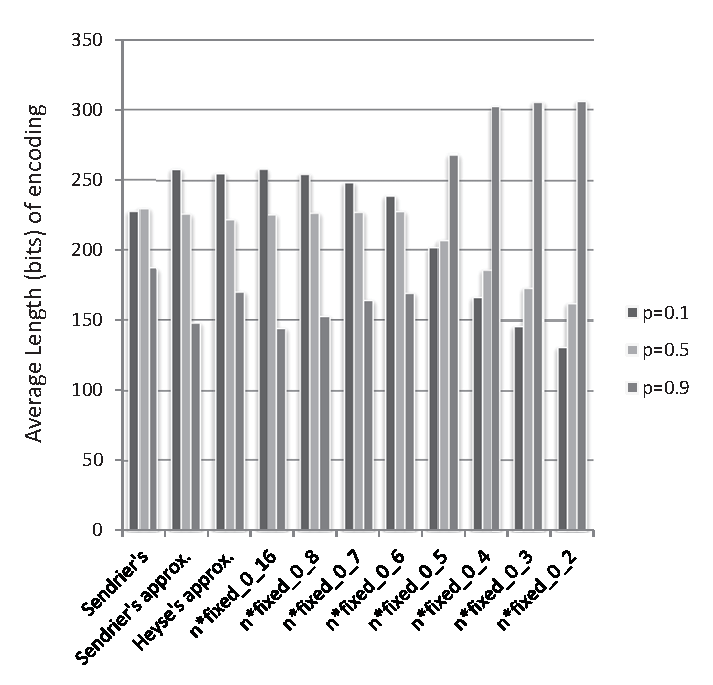
\includegraphics[width=\textwidth,height=.27\textheight]{./fig/best_d-10-38.eps}
\caption{$n=2^{10},t=38$}
\end{subfigure}
\hfill
\begin{subfigure}{.42\textwidth}\centering
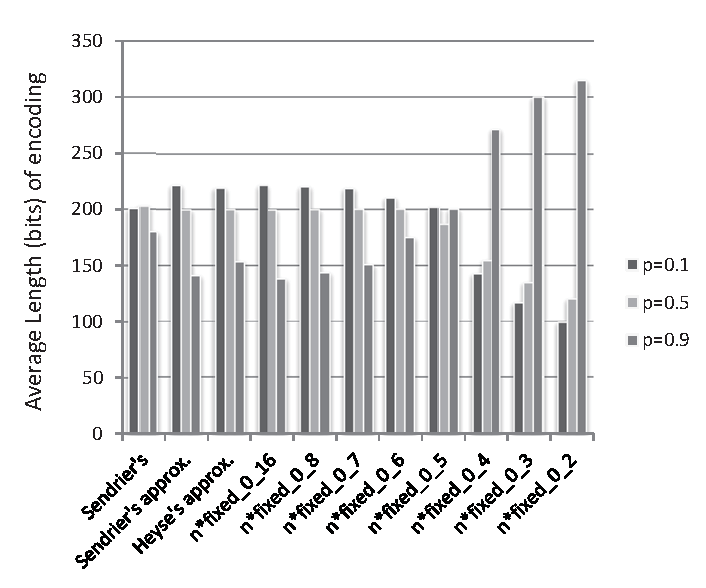
\includegraphics[width=\textwidth,height=.27\textheight]{./fig/best_d-11-27.eps}
\caption{$n=2^{11},t=27$}
\end{subfigure}
\hfill
\begin{subfigure}{.42\textwidth}\centering
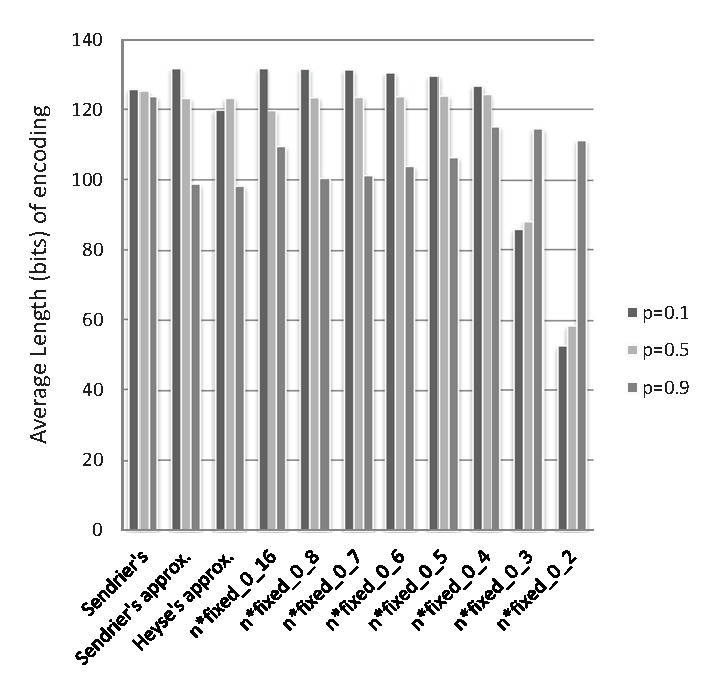
\includegraphics[width=\textwidth,height=.27\textheight]{./fig/best_d-16-9.eps}
\caption{$n=2^{16},t=9$}
\end{subfigure}
\hfill
\begin{subfigure}{.42\textwidth}\centering
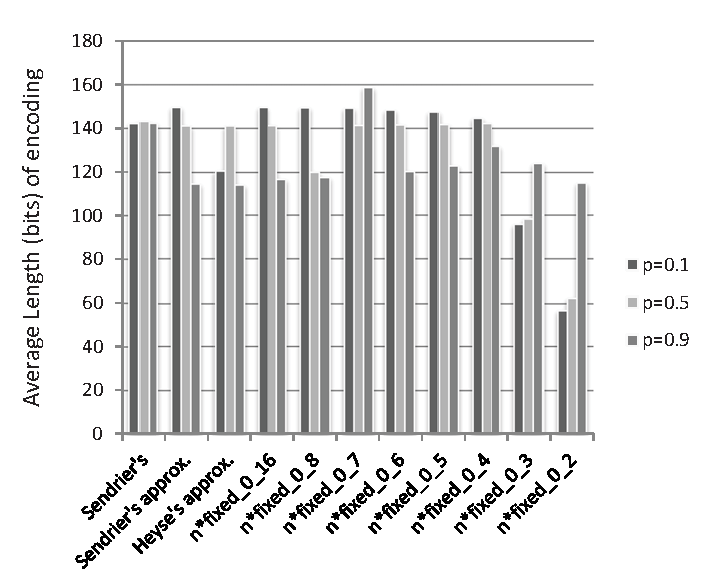
\includegraphics[width=\textwidth,height=.27\textheight]{./fig/best_d-18-9.eps}
\caption{$n=2^{18},t=9$}
\end{subfigure}
\hfill
\begin{subfigure}{.42\textwidth}\centering
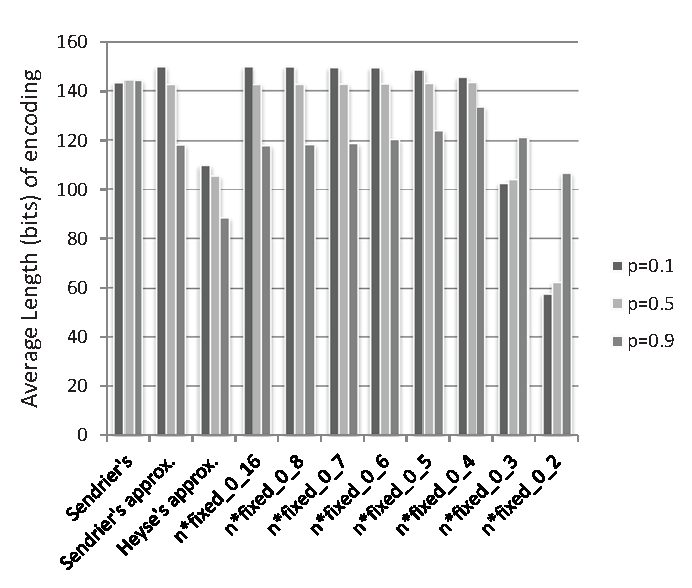
\includegraphics[width=\textwidth,height=.27\textheight]{./fig/best_d-20-8.eps}
\caption{$n=2^{20},t=8$}
\end{subfigure}
\caption{The performance of different methods for choosing the optimal $d$.
We have listed  five most frequently used sets of $(n, t)$  for the Niederreiter cryptosystem.
We have done three experiments for each $(n, t)$ in which the input binary message contains '1' with the probability $p=0.1$, $p=0.5$ and $p=0.9$ respectively.
The results of each experiment are obtained by running 10,000 different messages.
The X-axis lists different methods including Senderier's primitive\cite{sendrier2005encoding}, Senderier's approximation\cite{sendrier2005encoding},
Heyse's approximation\cite{heyse2012towards}  and our n*fixed\_0\_16 --- n*fixed\_0\_2. The Y-axis represents the average length (bits) of the input message read for
a successful constant weight encoding.}
\label{fig:best_d}
\end{figure*}


Figure~\ref{fig:best_d} describes the coding performances when we adjust the precision of $\theta[t]$.
Taken as whole, the $p=0.1$ group and $p=0.5$ group have a similar trend of average message length encoded as the arithmetic precision decreases:
The message length drops slightly from n*fixed\_0\_16 --- n*fixed\_0\_2 in consistency. On the contrary,
 $p=0.9$ group appears to be quite different where the numbers of bits read for a single constant weight coding first stay stable
 and then drop with the approximation precision decreasing. The numbers first keep stable because the loss of precision in $\theta[t]$ is comparatively trivial but if
 the precision drops too low, for instance, with fixed\_0\_2 representation $\theta[t]=0$ for $2\leq t \leq 38$ and hence $d=0$. It leads to a constant $n$ and small value of $i$
  in Algorithm~\ref{alg:encoding} forcing us to read more bits of input stream before the algorithm halts. According to the evaluation criteria mentioned in the last paragraph,
we compute the average length of the three types of plaintexts and identify the best approximation of $d$ from our proposal after analyzing the statistics obtained.
On the one hand,  the n*fixed\_0\_5 group outperforms at $(n=2^{10},t=38)$ and $(n=2^{11},t=27)$.
On the other hand, the n*fixed\_0\_4 group  beats the others at $(n=2^{16},t=9)$, $(n=2^{18},t=9)$  and $(n=2^{20},t=8)$.

% Note that often IEEE papers with subfigures do not employ subfigure
% captions (using the optional argument to \subfloat[]), but instead will
% reference/describe all of them (a), (b), etc., within the main caption.
% Be aware that for subfig.sty to generate the (a), (b), etc., subfigure
% labels, the optional argument to \subfloat must be present. If a
% subcaption is not desired, just leave its contents blank,
% e.g., \subfloat[].








% An example of a floating table. Note that, for IEEE style tables, the
% \caption command should come BEFORE the table and, given that table
% captions serve much like titles, are usually capitalized except for words
% such as a, an, and, as, at, but, by, for, in, nor, of, on, or, the, to
% and up, which are usually not capitalized unless they are the first or
% last word of the caption. Table text will default to \footnotesize as
% the IEEE normally uses this smaller font for tables.
% The \label must come after \caption as always.
%
%\newcommand{\tabincell}[2]{\begin{tabular}{@{}#1@{}}#2\end{tabular}}
\begin{table*}[!tbh]
% increase table row spacing, adjust to taste
\renewcommand{\arraystretch}{1.10}
 %if using array.sty, it might be a good idea to tweak the value of
 %\extrarowheight as needed to properly center the text within the cells
\caption{The coding performance of the optimal $d$ chosen from our approximation method}
\label{tab:best_d}
\centering
% Some packages, such as MDW tools, offer better commands for making tables
% than the plain LaTeX2e tabular which is used here.
\begin{tabular}{cccccccc}
\hline
\multirow{2}{*}{$n$} & \multirow{2}{*}{$t$} &\multirow{2}{*}{method}& \multicolumn{3}{c}{number of bits read} &\multirow{2}{*}{\tabincell{c}{coding efficiency}} &\multirow{2}{*}{\tabincell{c}{efficiency improved}}\\

    &  &           &  maximum & minimum & average       &    & \\
\hline
\multirow{4}{*}{$2^{10}$}    & \multirow{4}{*}{$38$}   &Sendrier's\cite{sendrier2005encoding}            &236 &164    &214.70  &93.19\% & --- \\
                            &                          &Sendrier's approx.\cite{sendrier2005encoding}       &263 &124    &210.45 &91.32\% & -1.98\% \\
		
                            &                          &Heyse's approx.\cite{heyse2012towards}       &261 &143    &210.73  &91.44\% &-1.85\%\\

                            &                          &\textbf{n*fixed\_0\_5}             &311  &183    &225.54   &97.89\%&\textbf{+5.05\%}\\

\hline
\multirow{4}{*}{$2^{11}$}    & \multirow{4}{*}{$27$}  & Sendrier's\cite{sendrier2005encoding}            &208&160    &194.46   &95.51\%& --- \\
                            &                          &Sendrier's approx.\cite{sendrier2005encoding}       &227 &119    &187.55 &92.11\% &-3.56\%\\
                            &                          &Heyse's approx.\cite{heyse2012towards}      &224&127    &190.96   &93.78\%&-1.80\%\\

                            &                          &\textbf{n*fixed\_0\_5}             &361&132    &196.30   &96.41\%&\textbf{+0.95\%}\\

\hline
\multirow{4}{*}{$2^{16}$}    & \multirow{4}{*}{$9$}  &  Sendrier's\cite{sendrier2005encoding}           &133       &113    &124.87   &99.50\%& --- \\
                            &                          &Sendrier's approx.\cite{sendrier2005encoding}       &133 &77    &117.80 &93.84\% &-5.10\%\\
                            &                          &Heyse's approx.\cite{heyse2012towards}     &133       &86   &116.34  &92.68\%&-6.83\%\\

                            &                          &\textbf{n*fixed\_0\_4}            &135       &95    &121.98   &97.20\%&\textbf{-2.37\%}  \\

\hline
\multirow{4}{*}{$2^{18}$}    & \multirow{4}{*}{$9$}  &  Sendrier's\cite{sendrier2005encoding}           &148       &132    &142.61   &99.38\%&---\\
                            &                          &Sendrier's approx.\cite{sendrier2005encoding}       &151 &91    &135.17 &94.18\% &-5.22\%\\
                            &                          &Heyse's approx.\cite{heyse2012towards}     &300       &101    &133.21   &92.81\%&-6.60\%\\

                            &                          &\textbf{n*fixed\_0\_4}            &154       &112    &139.64   &97.31\%&\textbf{-2.08\%}\\

\hline
\multirow{4}{*}{$2^{20}$}    & \multirow{4}{*}{$8$}  &  Sendrier's\cite{sendrier2005encoding}           &149      &135    &144.00   &99.52\%&---\\
                            &                          &Sendrier's approx.\cite{sendrier2005encoding}       &151 &99    &136.94 &94.64\% &-4.90\%\\
                            &                          &Heyse's approx.\cite{heyse2012towards}     &265      &17     &110.07    &76.07\%&-23.56\%\\

                            &                          &\textbf{n*fixed\_0\_4}            &158  &109    &140.81   &97.31\%&\textbf{-2.22\%}\\

\hline
\end{tabular}
\end{table*}


% Note that the IEEE does not put floats in the very first column
% - or typically anywhere on the first page for that matter. Also,
% in-text middle ("here") positioning is typically not used, but it
% is allowed and encouraged for Computer Society conferences (but
% not Computer Society journals). Most IEEE journals/conferences use
% top floats exclusively.
% Note that, LaTeX2e, unlike IEEE journals/conferences, places
% footnotes above bottom floats. This can be corrected via the
% \fnbelowfloat command of the stfloats package.



Table~\ref{tab:best_d} compares our proposed methods with the Sendrier's \cite{sendrier2005encoding},
Sendrier's original approximation using power of 2 \cite{sendrier2005encoding} and Heyse's table lookup approximation \cite{heyse2010low}.
From this table it is seen that our proposal gains  better coding efficiency than the original approximation and Heyse's approximation among all five parameter sets used for the Niederreiter scheme. Note that the average number of bits we have to read before producing the constant weight words is upper bound by
$log_2\binom{n}{t}$ and the thus the ratio of the average number read and the upper bound measures the coding efficiency \cite{sendrier2005encoding}. Additionally, our proposal even outperforms the Sendrier's method at two of these parameter sets --- $(n=2^{10},t=38)$ and $(n=2^{11},t=27)$
with 5.05\% and  0.95\% of improvements, respectively. It is also worth mentioning that for $(n=2^{16},t=9)$, $(n=2^{18},t=9)$  and $(n=2^{20},t=8)$, the performance of our proposal falls slightly behind with 2.37\%, 2.08\% and 2.22\% of loss when compared with the Sendrier's method, it nonetheless outruns Sendrier's approximation and Heyse's approximation. In particular, the performance of Heyse's approximation
becomes unfavourable with 23.56\% loss at $(n=2^{20},t=8)$ and we are pushing the limits of Heyse's method here
as the lower bits of $n$ are innegligible and cannot be removed with such large $n$.


\section{Proposed constant weight encoder and decoder}
\subsection{best\_d module}
\renewcommand{\arraystretch}{1.2}
\begin{table}[!htb]\centering
\caption{Encoding of $\theta[t]$}\label{tab:encode_theta}
\begin{minipage}{.48\textwidth}\centering
\begin{tabular}{ccc}
\hline
    value of $t$                &  $\theta[t]=(0.\theta_1\theta_2\theta_3\theta_4\theta_5)_2$\footnote[$\ast$]{This $\theta[t]$ is represented in fixed\_0\_5 form, e.g. $\theta[t]=\sum_{i=1}^{5}\theta_i\cdot 2^{-i}$. This format is used in $(n=2^{10},t=38)$ and $(n=2^{11},t=27)$.} & $\theta[t]=(0.\theta_1\theta_2\theta_3\theta_4)_2$\footnote[$\dagger$]{This $\theta[t]$ is represented in fixed\_0\_4 form, e.g. $\theta[t]=\sum_{i=1}^{4}\theta_i\cdot 2^{-i}$. This format is used in $(n=2^{16},t=9)$, $(n=2^{18},t=9)$ and $(n=2^{20},t=8)$.}\\
\hline
 $22\leq t\leq 38$  &  $00000$ & \multirow{2}{*}{N/A}\\
 $11\leq t\leq 21$  & $00001$  &\\
\hline
 $8\leq t\leq 10$  & $00010$  &\multirow{2}{*}{$0001$}\\
 $6\leq t\leq 7$  & $00011$  &\\
\hline
 $t = 5$  & $00100$  & \multirow{2}{*}{$0010$}    \\
 $t = 4$  & $00101$  &     \\
\hline
 $t = 3$  & $00110$  &  $0011$   \\
 $t = 2$  &$01001$   &  $0100$   \\
 $t = 1$  &$10000$   & $1000$    \\
\hline
\end{tabular}
\end{minipage}
\end{table}

\begin{table}[!htb]\centering
\renewcommand{\arraystretch}{1.2}
\caption{Decoding of $n\cdot\theta[t]$}\label{tab:decode_ntheta}
\begin{minipage}{.48\textwidth}\centering
\begin{tabular}{ccc}
\hline
     integer part of $n\cdot\theta[t]$          & value of $d$  & value of $u$\\
\hline
 $n\theta[t] > 2^{18}$  &  $2^{19}$ & $19$\\
 \hline
 $ 2^{17}< n\theta[t] \leq 2^{18}$  &  $2^{18}$ & $18$\\
 $ 2^{16}< n\theta[t] \leq 2^{17}$  &  $2^{17}$ & $17$\\
 $ 2^{15}< n\theta[t] \leq 2^{16}$  &  $2^{16}$ & $16$\\
 $ 2^{14}< n\theta[t] \leq 2^{15}$  &  $2^{15}$ & $15$\\
 $ 2^{13}< n\theta[t] \leq 2^{14}$  &  $2^{14}$ & $14$\\
 $ 2^{12}< n\theta[t] \leq 2^{13}$  &  $2^{13}$ & $13$\\
 $ 2^{11}< n\theta[t] \leq 2^{12}$  &  $2^{12}$ & $12$\\
 $ 2^{10}< n\theta[t] \leq 2^{11}$  &  $2^{11}$ & $11$\\
 $ 2^{9}< n\theta[t] \leq 2^{10}$  &  $2^{10}$ & $10$\\
 $ 2^{8}< n\theta[t] \leq 2^{9}$  &  $2^{9}$ & $9$\\
 $ 2^{7}< n\theta[t] \leq 2^{8}$  &  $2^{8}$ & $8$\\
 $ 2^{6}< n\theta[t] \leq 2^{7}$  &  $2^{7}$ & $7$\\
 $ 2^{5}< n\theta[t] \leq 2^{6}$  &  $2^{6}$ & $6$\\
 $ 2^{4}< n\theta[t] \leq 2^{5}$  &  $2^{5}$ & $5$\\
 $ 2^{3}< n\theta[t] \leq 2^{4}$  &  $2^{4}$ & $4$\\
 $ 2^{2}< n\theta[t] \leq 2^{3}$  &  $2^{3}$ & $3$\\
 $ 2< n\theta[t] \leq 2^{2}$  &  $2^{2}$ & $2$\\
 $ 1< n\theta[t] \leq 2$  &  $2$ & $1$\\
 \hline
 $ n\theta[t] \leq 1$  &  $1$ & $0$\\
\hline
\end{tabular}
\end{minipage}
\end{table}

The most critical arithmetic unit is the best\_d module which computes the best value of $d$ according to the input $n$ and $t$.
With our proposal of computation of $best\_d$, it consists of three stages performing the following task:
\begin{enumerate}
\item \textbf{compute $\theta[t]$ via a priority encoder.} As discussed in previous section, format fixed\_0\_5 is used to represent $\theta[t]$ for
$(n=2^{10},t=38)$ and $(n={2^{11},t=27})$ and fixed\_0\_4 is used for $(n=2^{16},t=9)$, $n={2^{18},t=9}$ and $n={2^{20},t=8}$. We find by analysis
that for some $t$, the value of $\theta[t]$ are identical. For instance, $\theta[6]=\theta[7]=(0.00011)_2=0.09375$ in fixed\_0\_5 format, shown in
Table~\ref{tab:encode_theta}. This observation drives us to exploit priority encoder to simplify the encoding of $\theta[t]$.

\item \textbf{compute $n\cdot \theta[t]$ via a fixed point multiplier.} We configured the Xilinx LogiCORE IP to implement high-performance,
optimized multipliers for different $n$ and $t$. The fractional part of the multiplication result is truncated and its integer part is
preserved for the next stage to process.

\item \textbf{output the value of $d$ and $u$.} Recall that the value of $n\cdot \theta[t]$ must be round to $d=2^u$. Here again another
priority encoder is used to decode the integer part of $n\cdot \theta[t]$. The detailed decoding process is listed in Table~\ref{tab:decode_ntheta}.
\end{enumerate}

Figure~\ref{fig:best_d} depicts our best\_d unit. This unit works in three stage pipelines. It first computes $\theta[t]$ and
then obtains $n\cdot\theta[t]$ using a multiplier. Finally, the value of $d$ would be determined by a priority decoder.
\begin{figure}[!htb]\centering
   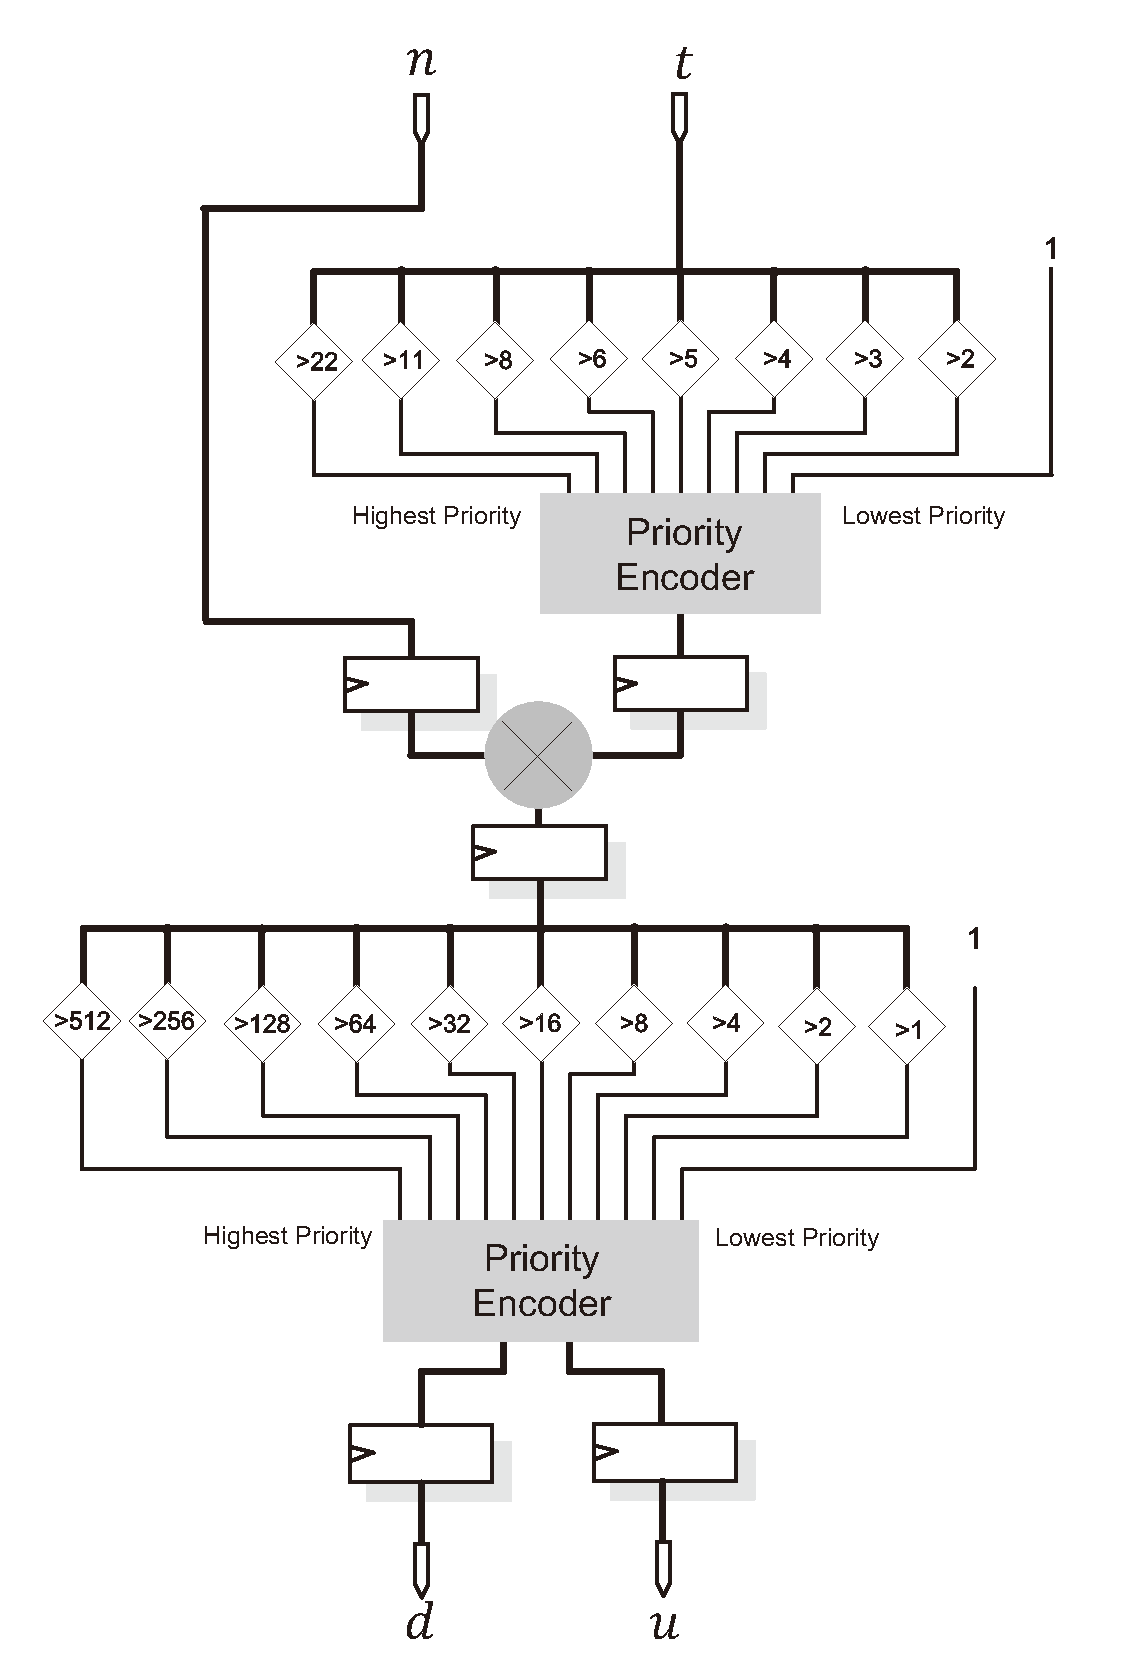
\includegraphics[width=0.40\textwidth]{./fig/best_d.eps}
   \caption{best\_d module for CW encoder and decoder. We list here the detailed configurations of $n=2^{11},t=27$ for demonstrative purpose.}
    \label{fig:best_d}
\end{figure}





\subsection{Bin2CW encoder}
Figure~\ref{fig:encoder} depicts the architecture of the proposed constant weight encoder.
Input binary message is passed inwards using a non-symmetric 8-to-1 FIFO which imitates the function of $\text{read}(B,1)$.
We use a serial-in-parallel-out shift register to perform $\text{read}(B,u), 0 \leq u\leq \lceil log_2(\frac{n}{2})\rceil$.
The proposed best\_d module is exploited here to compute the value of d. The values of $n$, $t$, $\delta$
are accordingly updated using three registers.

\begin{figure*}[!tbh]\centering
      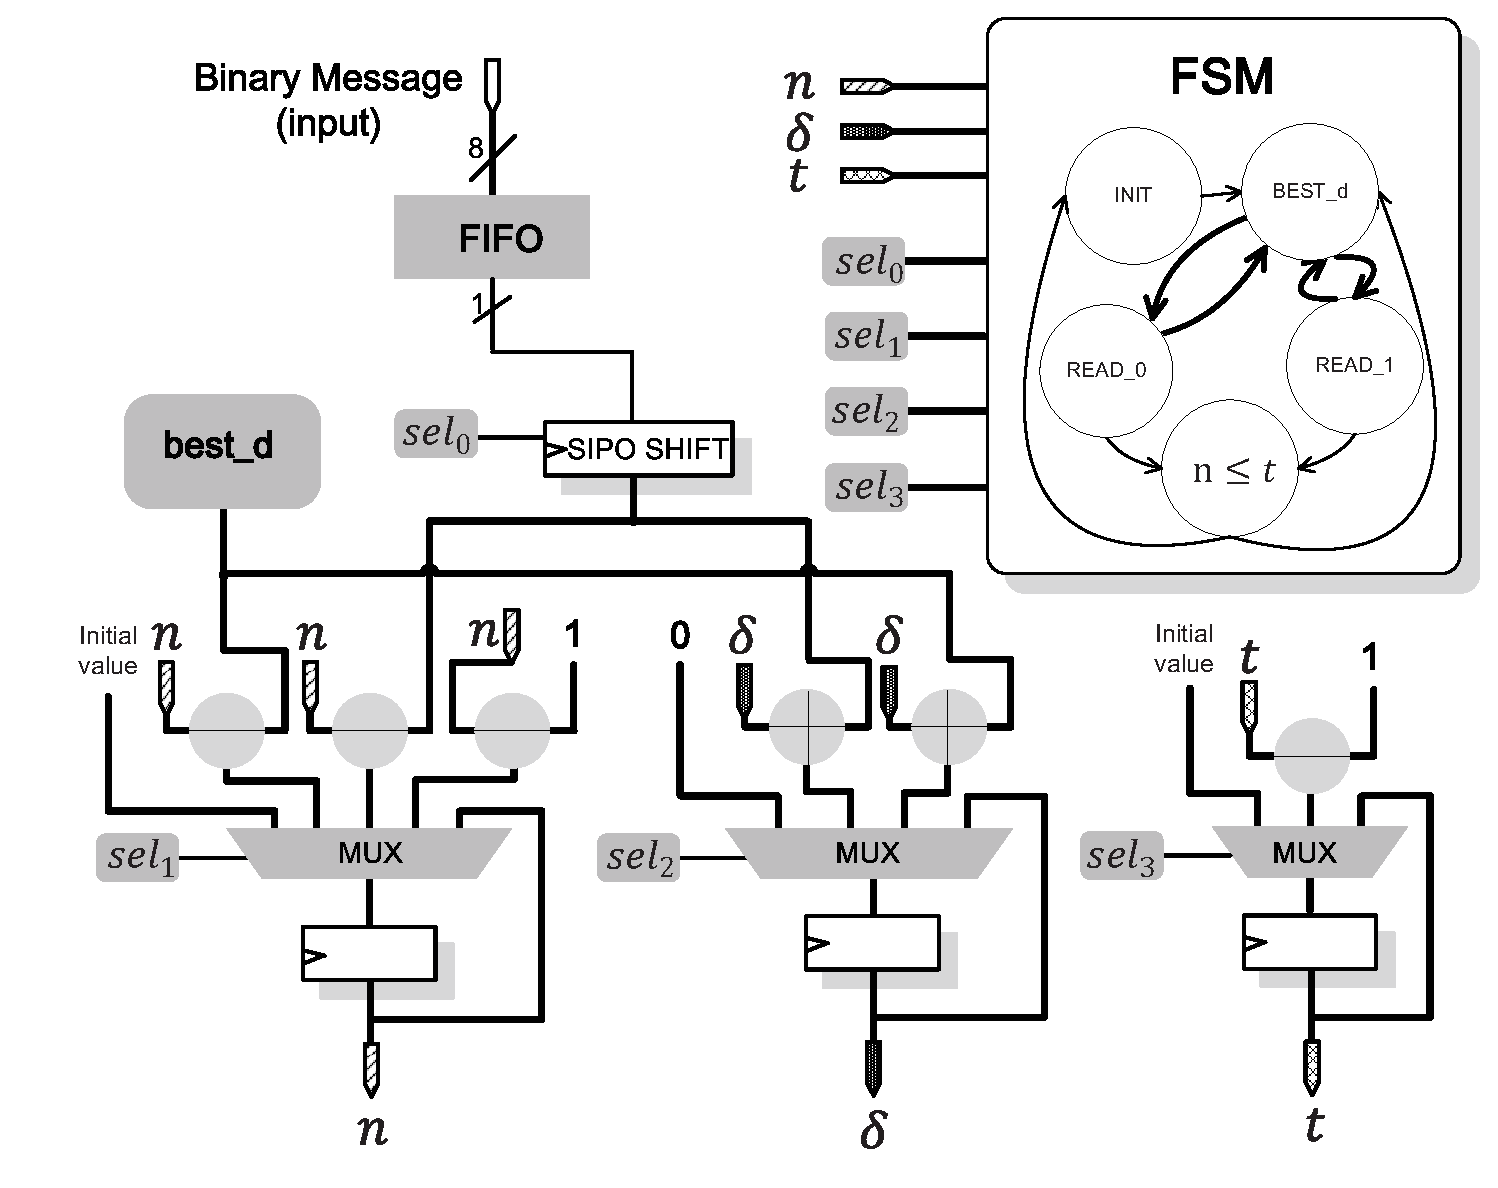
\includegraphics[width=0.65\textwidth]{./fig/encoder.eps}
  \caption{General architecture of CW encoder}\label{fig:encoder}
\end{figure*}

\subsection{CW2Bin decoder}
Figure~\ref{fig:decoder} depicts the architecture of the proposed constant weight decoder.
A m-to-m bit FIFO is used instead to transfer the input $t$-tuple word by word. This logic
is actually the bottle neck in the constant weight decoder when compared with the encoder. We similarly use
three registers to update the values of $n$, $t$, $\delta$. The major difference is that the shift register
here outputs the value of $\delta$ bit by bit as step~9 of Algorithm~\ref{alg:decoding} requires.

\begin{figure*}[!htb]\centering
      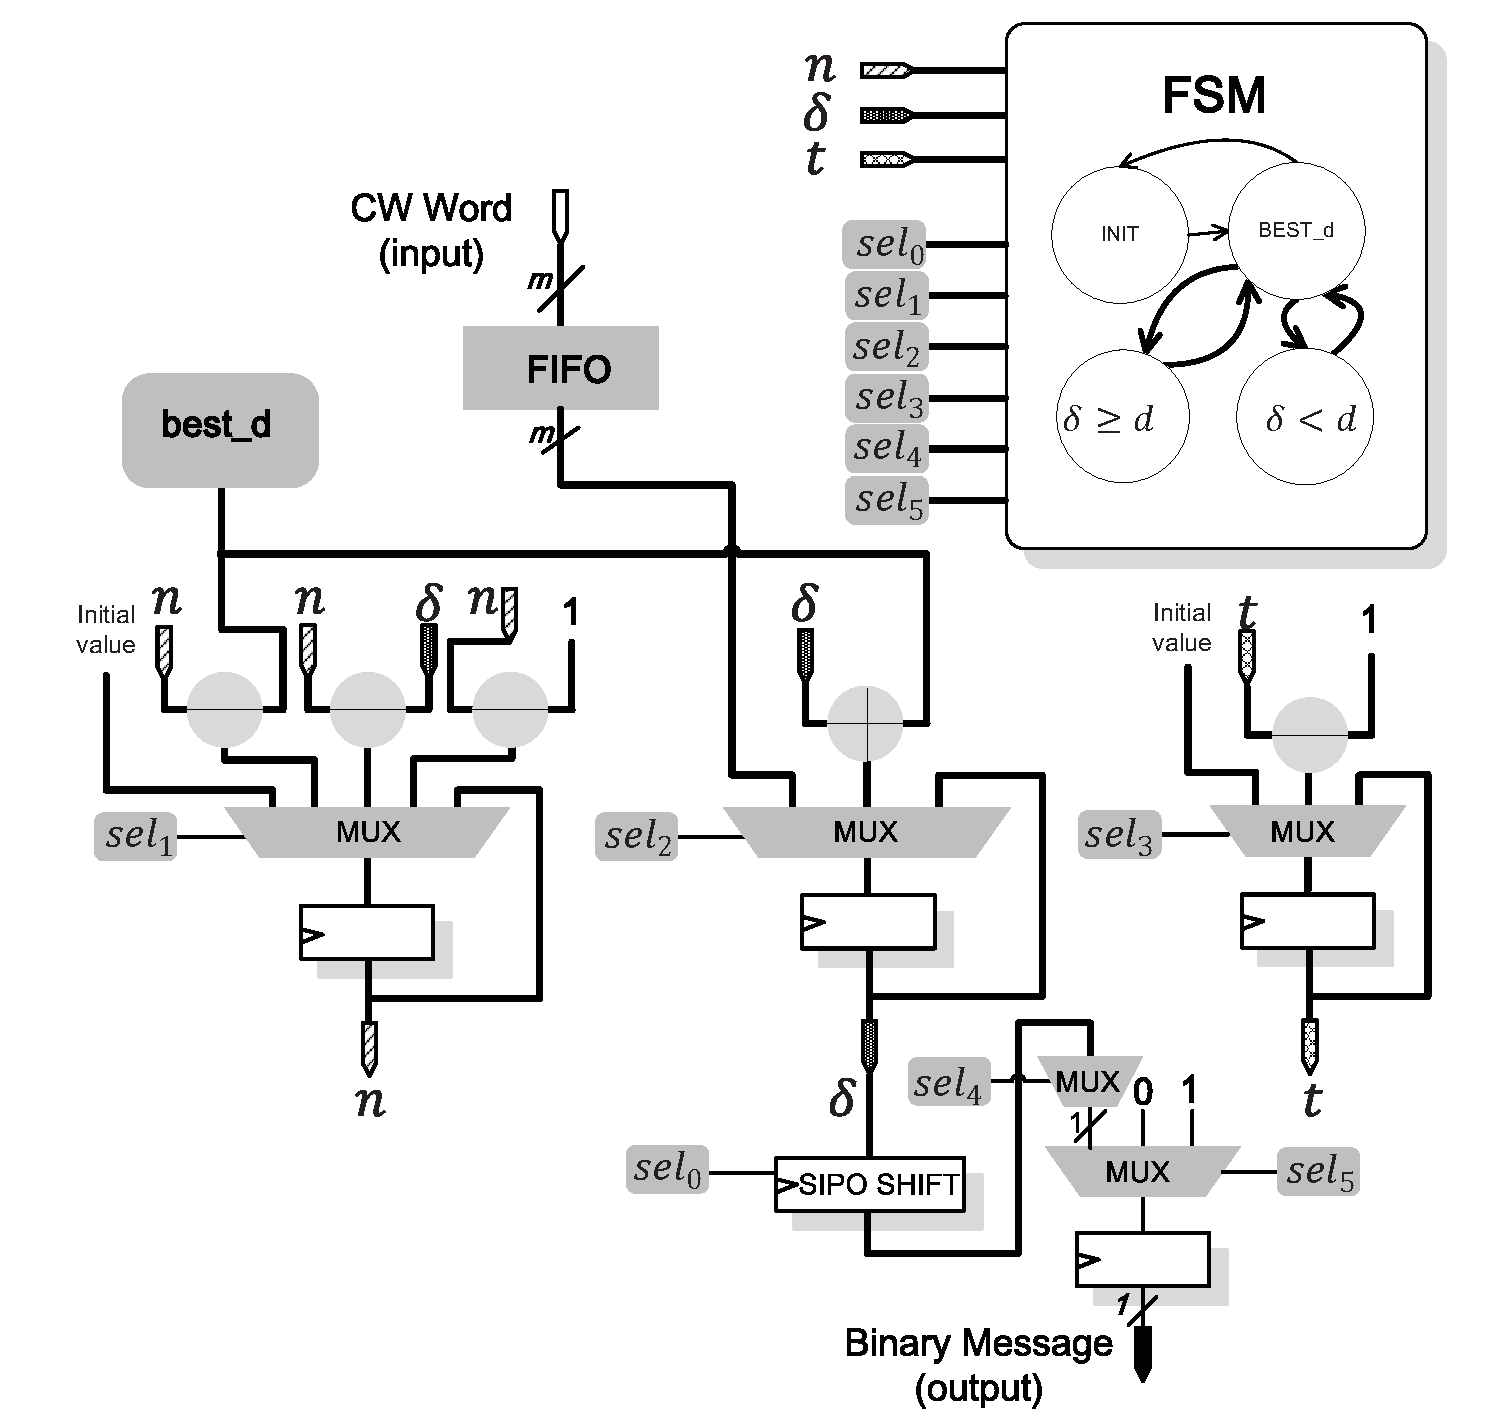
\includegraphics[width=0.65\textwidth]{./fig/decoder.eps}
  \caption{General architecture of CW decoder}\label{fig:decoder}
\end{figure*}

\section{Integrating with the Niederrieter encryptor}
In this section, we demonstrate how the proposed Bin2CW encoder can integrate with the Niederrieter encryptor for data encryption, shown
in Algorithm~\ref{alg:NiederreiterEncrypt}.

\begin{figure*}[!htb]\centering
   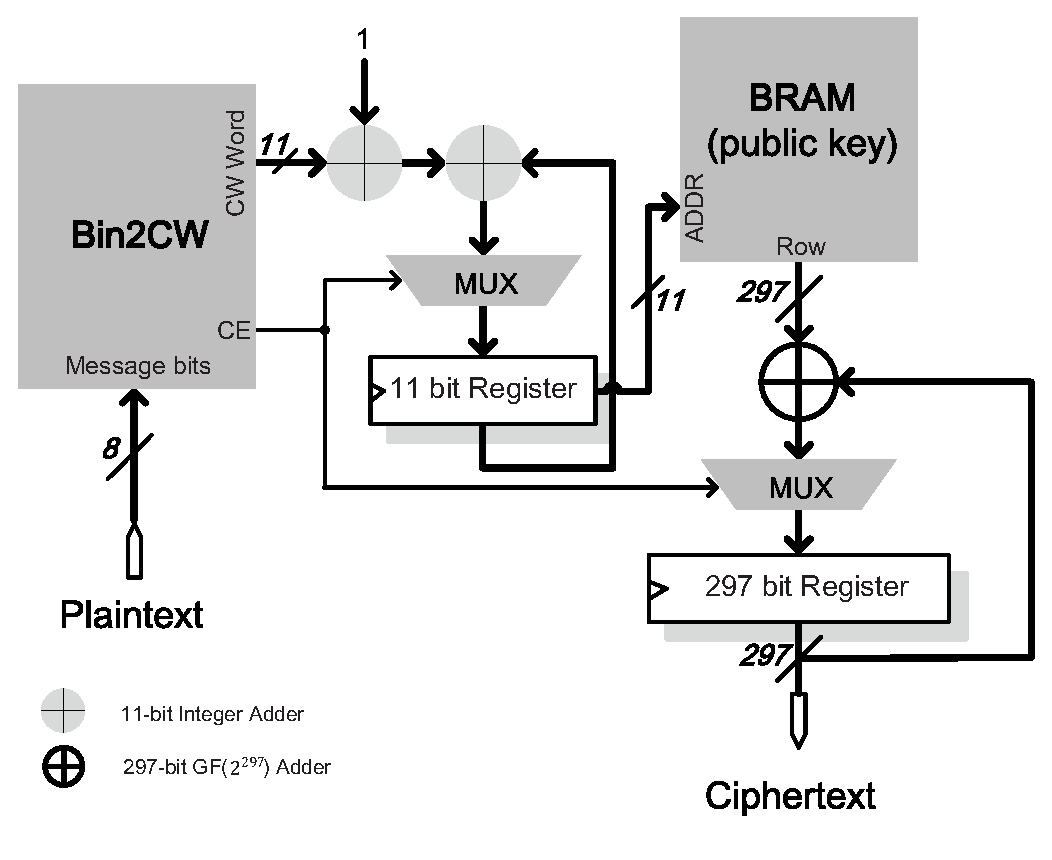
\includegraphics[width=0.65\textwidth]{./fig/encryptor.eps}
   \caption{Block diagram of the Niederrieter encryptor.}
    \label{fig:encryptor}
\end{figure*}

\begin{algorithm}[!htb]	
	\DontPrintSemicolon % Some LaTeX compilers require you to use \dontprintsemicolon instead
	\KwIn{message vector $m$, public key $pk=$\{${\hat H}$,$t$\} where $\hat H$ is an $n$ by $mt$ matrix}
	\KwOut{ciphertext $c$}
	Bob encodes the message $m$ as a binary matrix/vector of length $n$ and weight at most $t$.\;
    Bob computes the ciphertext as $c = {\hat H}m^T$, $m^T$ is the transpose of matrix $m$.\;
    \Return {$c$}
	\caption{Niederreiter Message Encryption, referenced from \cite{hu2015application}}\label{alg:NiederreiterEncrypt}
\end{algorithm}

The Bin2CW encoder is used to perform the first step in this algorithm. Recall that Bin2CW encoder returns a $t$-tuple of integers
$(\delta_1,\ldots,\delta_t)$, which records the distance between consecutive '1's in the string. However such $t$-tuple cannot
be directly transferred to compute the ciphertext. We believe that the way Heyse \textit{et al.}\cite{heyse2012towards} encrypts $c = {\hat H}m^T$ with
$m=(\delta_1,\ldots,\delta_t)$  is incorrect due to two reasons:
\begin{enumerate}
\item It is very likely that $\delta_i = \delta_j$ where $i\neq j$ such that the number of errors are less than $t$ and
it is assumed to be insecure from cryptoanalysis points of view.
\item $(\delta_1,\ldots,\delta_t)$ returns the integer ranging from $0$ to $n-t$ but the constant weight word
exactly ranges from $0$ to $n$. That is to say, the last $t$ rows of the public key $\hat{H}^T$ are never used.
\end{enumerate}

To fix this flaw from \cite{heyse2012towards}, we propose to return the `real' constant weight binary words of length $n$
and Hamming weight $t$. Suppose the constant weight are represented by $(i_1,\ldots,i_t)$, the coordinates of the `1's in ascending
order, then we compute $i_1=\delta_1$, $i_2=\delta_2+i_1+1$, $\ldots$, $i_t=\delta_t+i_{t-1}+1$ as the input of the second step, Algorithm~\ref{alg:NiederreiterEncrypt}.



Figure~\ref{fig:encryptor} depicts our revised version of Niederreiter encryption unit on the basis of \cite{heyse2012towards}.
The public key $\hat{H}^T$ is stored in an internal BRAM and row-wise addressed by the output of the 11 bit register. Two 11-bit
integer adders are embedded to convert $(\delta_1,\ldots,\delta_t)$ to $(i_1,\ldots,i_t)$ which are eventually stored in the 11 bit register.
The vector-matrix multiplication in step 2, Algorithm~\ref{alg:NiederreiterEncrypt} is equivalent to a XOR operation of selected rows
of $\hat{H}^T$, denoted here as a $GF(2^{297})$ adder in this figure. It is also worth mentioning that the vector-matrix multiplication
work concurrently with CW encoding: Whenever a valid $i_k$ has been computed, it is  transferred to the $GF(2^{297})$ adder
summing up the selected rows. After the last $i_t$ has been computed, the last indexed row of $\hat{H}^T$ also has been added to the sum.
This sum, stored in the 297-bit register, is now available as the ciphertext.

\section{Results and comparisons}
\begin{table*}[!htb]\centering
    \caption{Compact implementations of CW encoder and decoder on Xilinx Virtex-6 FPGA}\label{tab:result}
\begin{subtable}[t]{0.95\linewidth}\centering
    \caption{$n=2^{10}, t=38$}
    \begin{tabular}{cccccccc}\hline
    &   Algorithm & Platform & \tabincell{c}{Area\\{}[slices]} &\tabincell{c}{Memory blocks\\{}[$36+18$ Kb RAM]} & \tabincell{c}{Frequency\\{}[MHz]} & \tabincell{c}{Throughout\\{}[Mbps]} & \tabincell{c}{Coding\\efficiency}\\
    \hline
    \multirow{2}{*}{\textbf{This work}} & Bin2CW, new approx. & \multirow{2}{*}{Xilinx xc6vlx240t} & 74 & 0+1 & 330  & 160.2 &\multirow{2}{*}{97.89\%}\\
                                        & CW2Bin, new approx. & & 79 & 0+1 & 330 & 148.1 & \\
    \hline
    \multirow{2}{*}{Heyse \textit{et al.}\cite{heyse2012towards}} & Bin2CW, Heyse's approx. & \multirow{2}{*}{Xilinx xc6vlx240t} & 110 & 0+1 & 310  &178.8 & \multirow{2}{*}{91.44\%}\\
                                        & CW2Bin, Heyse's approx. & & 88 & 0+1 & 310 & 162.1&  \\

    \hline
    \end{tabular}
\end{subtable}
\vspace{1.5em}

\begin{minipage}{\textwidth}\centering
\begin{subtable}[t]{0.95\linewidth}\centering
    \caption{$n=2^{11}, t=27$}
    \begin{tabular}{cccccccc}\hline
        &   Algorithm & Platform & \tabincell{c}{Area\\{}[slices]} & \tabincell{c}{Memory blocks\\{}[$36+18$Kb RAM]} & \tabincell{c}{Frequency\\{}[MHz]} & \tabincell{c}{Throughout\\{}[Mbps]}& \tabincell{c}{Coding\\efficiency}\\
    \hline
    \multirow{2}{*}{\textbf{This work}} & Bin2CW, new approx. & \multirow{2}{*}{Xilinx xc6vlx240t} & 91 & 0+1 & 350 & 187.2 &\multirow{2}{*}{96.41\%}\\
                                        & CW2Bin, new approx. &  & 95 & 0+1 & 340 & 168.6&\\

    \hline
    \multirow{2}{*}{Heyse \textit{et al.}\cite{heyse2012towards} } & Bin2CW, Heyse's approx. & \multirow{2}{*}{Xilinx xc6vlx240t} & 118 & 0+1 &340  &208.4 &\multirow{2}{*}{93.78\%}\\
                                        & CW2Bin, Heyse's approx. & & 110 & 0+1 & 340 &164.6 & \\

    \hline
    \multirow{2}{*}{Sendrier\cite{sendrier2005encoding}\footnote[$\ast$]{Sendrier implemented a different but very close parameter set $n=2^{11},t=30$. We also put it here for reference.}} & Bin2CW, original & \multirow{2}{*}{Intel Pentium 4} &\multirow{2}{*}{---}  & \multirow{2}{*}{---} & \multirow{2}{*}{2400} & 17.3 &95.51\%\\
                                        & Bin2CW, approximate & &  &  &  & 33.0 & 92.11\%\\

    \hline
    \end{tabular}
\end{subtable}
\end{minipage}
\vspace{1.5em}

\begin{subtable}[t]{0.95\linewidth}\centering
    \caption{$n=2^{16}, t=9$}
    \begin{tabular}{cccccccc}\hline
    &   Algorithm & Platform & \tabincell{c}{Area\\{}[slices]} & \tabincell{c}{Memory blocks\\{}[$36+18$ Kb RAM]} & \tabincell{c}{Frequency\\{}[MHz]} & \tabincell{c}{Throughout\\{}[Mbps]} & \tabincell{c}{Coding\\efficiency}\\
    \hline
     \multirow{2}{*}{\textbf{This work}} & Bin2CW, new approx. & \multirow{2}{*}{Xilinx xc6vlx240t} & 103 & 0+1 & 440 &316.1 & \multirow{2}{*}{97.20\%}\\
                                        & CW2Bin, new approx. &  & 109 & 0+1 & 310 &212.9 & \\

    \hline
    \multirow{2}{*}{Heyse \textit{et al.}\cite{heyse2012towards}} & Bin2CW, Heyse's approx. & \multirow{2}{*}{Xilinx xc6vlx240t} & 90 & 10+3 & 240 &182.3&\multirow{2}{*}{92.68\%}\\
                                        & CW2Bin, Heyse's approx. & & 90 & 10+3 & 230 & 170.3&\\

    \hline
    \multirow{2}{*}{Sendrier\cite{sendrier2005encoding}} & Bin2CW, original & \multirow{2}{*}{Intel Pentium 4} &\multirow{2}{*}{---}  & \multirow{2}{*}{---} & \multirow{2}{*}{2400} &18.3 &99.50\%\\
                                        & Bin2CW, approximate & &  &  &  &22.0 & 93.84\%\\

    \hline
    \end{tabular}
\end{subtable}
\vspace{1.5em}

\begin{subtable}[t]{0.95\linewidth}\centering
    \caption{$n=2^{18}, t=9$}
    \begin{tabular}{cccccccc}\hline
    &   Algorithm & Platform & \tabincell{c}{Area\\{}[slices]} & \tabincell{c}{Memory blocks\\{}[$36+18$Kb RAM]} & \tabincell{c}{Frequency\\{}[MHz]} & \tabincell{c}{Throughout\\{}[Mbps]} & \tabincell{c}{Coding\\efficiency}\\
    \hline
    \multirow{2}{*}{\textbf{This work}} & Bin2CW, new approx. & \multirow{2}{*}{Xilinx xc6vlx240t} & 138 & 0+1 & 410 & 295.5 &\multirow{2}{*}{97.31\%}\\
                                        & CW2Bin, new approx. &  & 118 & 0+1 & 320 & 219.5 &\\

    \hline
    \multirow{2}{*}{Heyse \textit{et al.}\cite{heyse2012towards}} & Bin2CW, Heyse's approx. & \multirow{2}{*}{Xilinx xc6vlx240t} & 94 & 40+3 & 170& 106.0&\multirow{2}{*}{92.81\%} \\
                                        & CW2Bin, Heyse's approx. & & 93 & 40+3 & 180 &104.9& \\

    \hline
    \end{tabular}
\end{subtable}
\vspace{1.5em}

\begin{subtable}[t]{0.95\linewidth}\centering
    \caption{$n=2^{20}, t=8$}
    \begin{tabular}{cccccccc}\hline
    &   Algorithm & Platform & \tabincell{c}{Area\\{}[slices]} & \tabincell{c}{Memory blocks\\{}[$36+18$Kb RAM]} & \tabincell{c}{Frequency\\{}[MHz]} & \tabincell{c}{Throughout\\{}[Mbps]} & \tabincell{c}{Coding\\efficiency}\\
    \hline
     \multirow{2}{*}{\textbf{This work}} & Bin2CW, new approx. & \multirow{2}{*}{Xilinx xc6vlx240t} & 156 & 0+1 & 370 & 284.9 &\multirow{2}{*}{97.31\%}\\
                                        & CW2Bin, new approx. &  & 122 & 0+1 & 300 & 222.7 & \\

    \hline
    \multirow{2}{*}{Heyse \textit{et al.}\cite{heyse2012towards}} & Bin2CW, Heyse's approx. & \multirow{2}{*}{Xilinx xc6vlx240t} & 124 & 160+3 & 130&96.6 & \multirow{2}{*}{76.07\%}\\
                                        & CW2Bin, Heyse's approx. & & 125 & 160+3 & 130& 98.8 &\\

    \hline
    \end{tabular}
\end{subtable}
\end{table*}

We captured our constant weight coding architecture in the Verilog language and prototyped our design on Xilinx Virtex-6 FPGA (Table~\ref{tab:result}).
To the best of our knowledge, the only compact implementations of constant weight coding have been proposed by Heyse \textit{et al.}\cite{heyse2012towards}.
Their light weight architecture is generally identical to ours except the design of best\_d module. Their best\_d module works in two pipeline stages:
In the first stage it retrieves the value of $u$ by table lookup. Then in the second stage it outputs $d$ according to the value of $u$ using
a simple decoder. Comparatively, our best\_d module has three stages of pipeline and thus it leads to
a lower throughput but our architectures are smaller and improve the area-time tradeoff of the constant weight coding implementations proposed
by Heyse \textit{et al.}\cite{heyse2012towards}, shown in Table~\ref{tab:result}. In particular, we use only one $18Kb$ memory block
for all parameter sets of our experiments.

We also observe  that in our designs, the memory footprint does not increase and the high clock frequency also maintains as the parameters grow. This is because the main difference among encoders or decoders with different parameters $n$ and $t$ is the operand size of multiplier embedded in the best\_d module, which grows logarithmically from $10 bit\times5bit$ to $20bit\times 4bit$. On the other hand, the memory overhead of Heyse's implementations grow linearly with $n$ and might be problematic when $n$ is large as aforementioned. To show this, we re-implemented Heyse's work for  $(n=2^{16}, t=9)$, $(n=2^{18},t=9)$ and $(n=2^{20},t=8)$. The experimental results verifies this point.
Additionally, another negative side effect of heavy memory overhead is that the working frequency of circuits drops rapidly as shown in Table~\ref{tab:result}. For small parameters (a) and (b), the lookup table in Heyse's design could be made of distributed memory (LUT) and therefore has
little impact on frequency. However for large parameters (c), (d) and (e), such look up table can no longer be instantized as LUTs because Xilinx Virtex-6 distributed memory generator only allows maximum data depth of 6,5536. We instead use block memory outside the FPGAs to construct the table and this accordingly leads to  slower speed due to relatively far and complicated routing. This block memory is the real bottleneck of
Heyse's work as $n$ grows.

We finally implemented the Niederreiter encryptor, a cryptographic application where constant weight coding is used exactly as mentioned in
Section~5. Table~\ref{table:encryptor_result} compares our work with the state of art\cite{heyse2012towards}. Our new implementation is the most compact one with better area-time tradeoffs.
We use the same block memory as \cite{heyse2012towards} did where $16\times 36$Kb + $1\times 18$Kb RAMs are utilized to store the public key matrix $\hat{H}$,
and one $18$Kb RAM for the 8-to-1 FIFO within the constant weight encoder.

 \begin{table}[!htb]\centering
 \renewcommand{\arraystretch}{1.4}
 \begin{minipage}{.5\textwidth}\centering
    \caption{FPGA Implementation results of Niederreiter encryption with $n=2048, t=27$ compared with~\cite{heyse2012towards} after PAR}
    \label{table:encryptor_result}
    \begin{tabular}{ l c c}
    \hline
         Aspect (Virtex6-VLX240) & Niederreiter~\cite{heyse2012towards} & \textbf{This work}  \\
    \hline
         Slices         & 315    & 183   \\
         LUTs           & 926   & 505 \\
         FFs            & 875   & 498 \\
         BRAMs          & 17    & 18\footnote[$\ast$]{We used $16\times$36Kb RAMs and $2\times$16Kb RAMs} \\
    \hline
        Frequency       & 300 MHz  &340 MHz \\
    \hline
    CW Encode $e$ = Bin2CW($m$) &     $\approx 200$ cycles          & $349.1$ cycles   \\
    Encrypt $c = e\cdot \hat{H}$ &    $\approx 200$ cycles           & $352.1$ cycles   \\
    \hline
    \end{tabular}
\end{minipage}
\end{table}

\section{Conclusion}
We proposed a new method of determining the optimal value d in constant weight coding.
This method enabled a more compact yet efficient implementation of constant weight encoder
and decoder for resource-constrained computing systems. Afterwards, we exploited
this new encoder to implement the Niederreiter encryptor on a Xilinx device.
For the time being, our design is the most compact one for any of the code-based encryption
schemes.



% if have a single appendix:
%\appendix[Proof of the Zonklar Equations]
% or
%\appendix  % for no appendix heading
% do not use \section anymore after \appendix, only \section*
% is possibly needed

% use appendices with more than one appendix
% then use \section to start each appendix
% you must declare a \section before using any
% \subsection or using \label (\appendices by itself
% starts a section numbered zero.)
%


%\appendices
%\section{Proof of the First Zonklar Equation}
%Appendix one text goes here.
%
%% you can choose not to have a title for an appendix
%% if you want by leaving the argument blank
%\section{}
%Appendix two text goes here.


% use section* for acknowledgment
\ifCLASSOPTIONcompsoc
  % The Computer Society usually uses the plural form
  \section*{Acknowledgments}
\else
  % regular IEEE prefers the singular form
  \section*{Acknowledgment}
\fi


The authors would like to thank...


% Can use something like this to put references on a page
% by themselves when using endfloat and the captionsoff option.
\ifCLASSOPTIONcaptionsoff
  \newpage
\fi



% trigger a \newpage just before the given reference
% number - used to balance the columns on the last page
% adjust value as needed - may need to be readjusted if
% the document is modified later
%\IEEEtriggeratref{8}
% The "triggered" command can be changed if desired:
%\IEEEtriggercmd{\enlargethispage{-5in}}

% references section

% can use a bibliography generated by BibTeX as a .bbl file
% BibTeX documentation can be easily obtained at:
% http://mirror.ctan.org/biblio/bibtex/contrib/doc/
% The IEEEtran BibTeX style support page is at:
% http://www.michaelshell.org/tex/ieeetran/bibtex/
\bibliographystyle{IEEEtran}
% argument is your BibTeX string definitions and bibliography database(s)
\bibliography{IEEEabrv,./reference}
%
% <OR> manually copy in the resultant .bbl file
% set second argument of \begin to the number of references
% (used to reserve space for the reference number labels box)


% biography section
%
% If you have an EPS/PDF photo (graphicx package needed) extra braces are
% needed around the contents of the optional argument to biography to prevent
% the LaTeX parser from getting confused when it sees the complicated
% \includegraphics command within an optional argument. (You could create
% your own custom macro containing the \includegraphics command to make things
% simpler here.)
%\begin{IEEEbiography}[{\includegraphics[width=1in,height=1.25in,clip,keepaspectratio]{mshell}}]{Michael Shell}
% or if you just want to reserve a space for a photo:

%\begin{IEEEbiography}{Michael Shell}
%Biography text here.
%\end{IEEEbiography}

% if you will not have a photo at all:
%\begin{IEEEbiographynophoto}{John Doe}
%Biography text here.
%\end{IEEEbiographynophoto}

% insert where needed to balance the two columns on the last page with
% biographies
%\newpage

%\begin{IEEEbiographynophoto}{Jane Doe}
%Biography text here.
%\end{IEEEbiographynophoto}

% You can push biographies down or up by placing
% a \vfill before or after them. The appropriate
% use of \vfill depends on what kind of text is
% on the last page and whether or not the columns
% are being equalized.

%\vfill

% Can be used to pull up biographies so that the bottom of the last one
% is flush with the other column.
%\enlargethispage{-5in}



% that's all folks
\end{document}


